

%!TEX root = ../thesis.tex
%******************************************************************************
\chapter[Conceptual Framework]{A Conceptual Framework for Feedback-Controlled Bulk Data Processing Systems}\label{ch:conceptual_framework}

%******************************************************************************
\section{Introduction} 

The concept for an adaptive Middleware for bulk data processing presented in chapter \ref{ch:adaptive_middleware} describes the ``What'' (what needs to be done) but not the ``How'' (how should it be done).

The design, implementation and operation of such a system differs from common approaches to implement enterprise systems:
\begin{itemize}
	\item There are specific activities or tasks needed to implement the feedback-control subsystem.
	\item There are different roles needed with different skills.
	\item There are different tools needed to aid the design and development of such as system.
\end{itemize}

Developing software is a complex process, the quality of a software product depends on the people, the organisation and procedures used to create and deliver it \citep{Fuggetta:2000ds}.
In order to guide the implementation of an adaptive system for bulk data processing, a conceptual framework is needed. It defines artifacts, roles, tasks and their dependencies to describe the necessary steps for design, implementation and operation of a system described in Chapter \ref{ch:adaptive_middleware}.

Figure \ref{fig:ch6_overview} shows an overview of the conceptual framework. It is organized among the phases plan, build and run. Each phase contains tasks, which are relevant for each phase:
\begin{itemize}
	\item Design: Defining Service interfaces, defining aggregation rules, defining transports, defining integration architecture
	\item Implementation: Service implementation, Service Optimisation
	\item Operation: controller tuning, monitoring
\end{itemize}

\begin{figure}
	[htpb] \centering 
	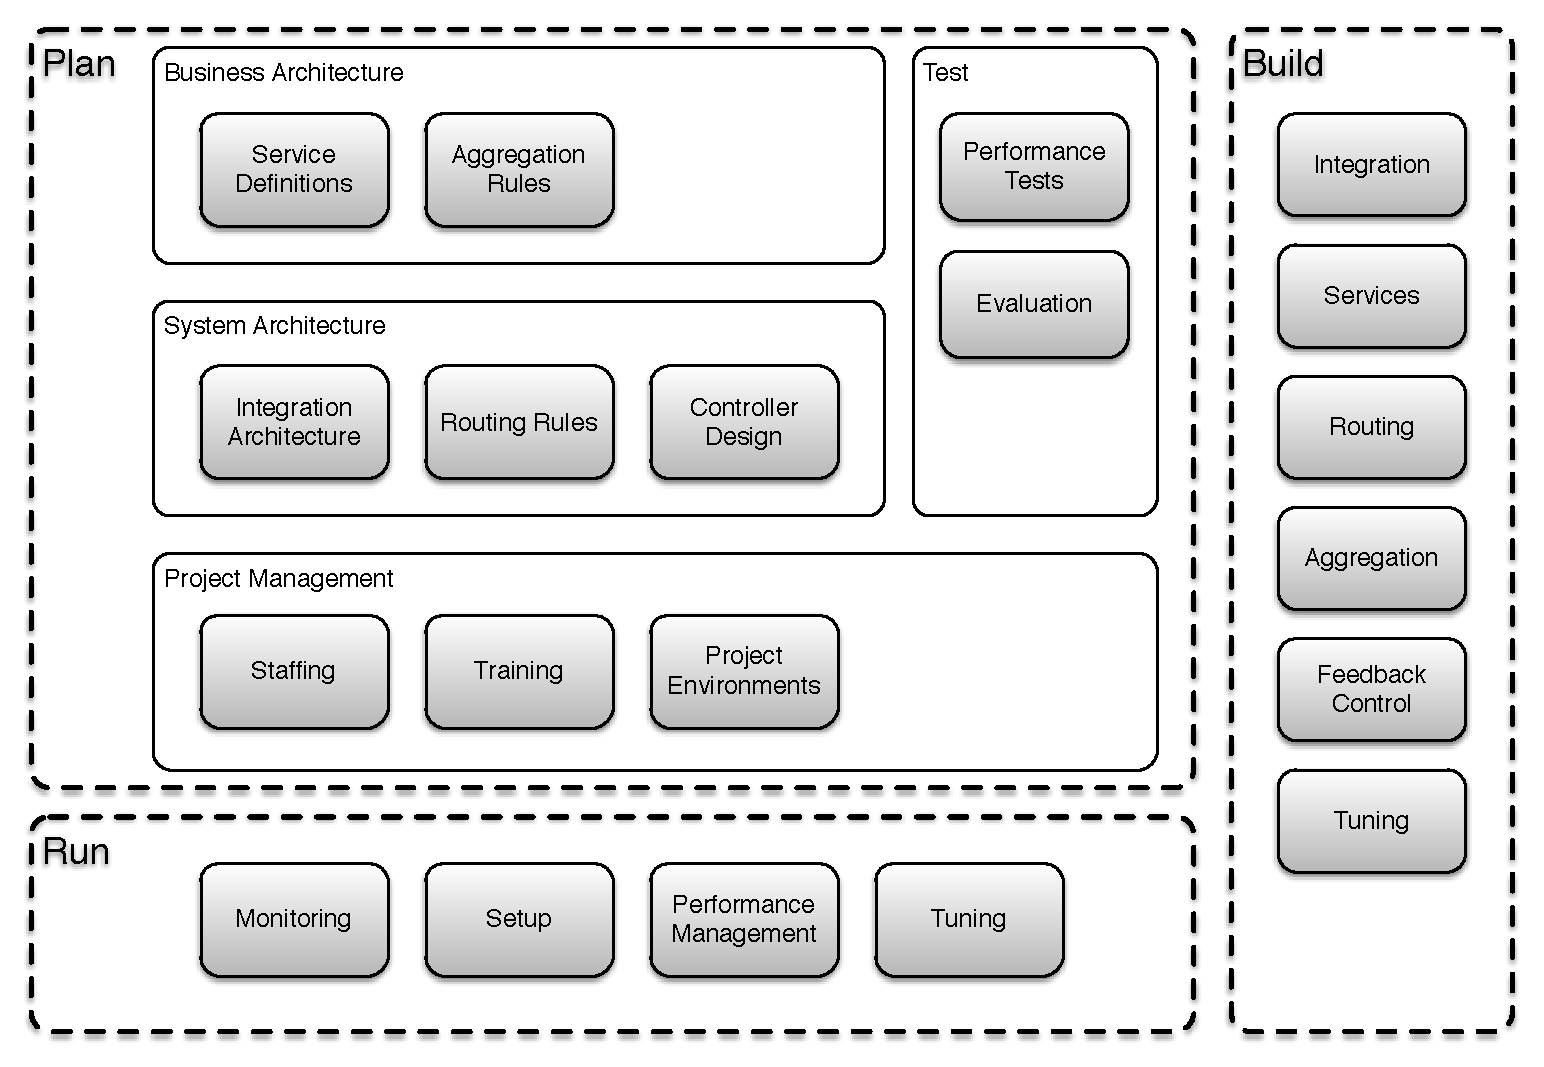
\includegraphics[width=\textwidth]{ch6_overview} \caption{Overview of Conceptual Framework} \label{fig:ch6_overview} 
\end{figure}


The conceptual framework only describes concepts that are specific to the design and implementation of an Adaptive Middleware as described in the previous chapter. It does not describe common concepts for softwar development.

This chapter is organised as follows:

\begin{itemize}
	\item Section \ref{sec:ch6_metamodel} describes the metamodel of the conceptual framework.
	\item The entities of the process model, roles, tasks, artifacts and tools, are described in the Sections \ref{sec:ch6_roles}, \ref{sec:ch6_tasks}, \ref{sec:ch6_artifacts} and \ref{sec:ch6_tools}.
	\item Section \ref{sec:ch6_other_frameworks} describes how the conceptual framework can be used with other architectural frameworks and software development methodologies such as TOGAF, \acf{RUP} and Scrum.
	\item Section \ref{sec:ch6_related_work} discusses other related approaches and work.
	\item Finally, this chapter concludes with a summary and a discussion of the presented conceptual framework (see Section \ref{sec:ch6_summary}).
\end{itemize}

\section{Metamodel}
\label{sec:ch6_metamodel}
The conceptual framework consists of the following entities, as shown in Figure \ref{fig:ch6_metamodel}:
\begin{itemize}
	\item \textbf{Phase}\\
	Phases correspond to the different phases of an software development process, such as design, implementation and operations and contain the relevant tasks.
	\item \textbf{Task}\\
	Tasks represent the activities of the development process. A task
	\begin{itemize}
		\item is contained in a phase
		\item is processed by a role
		\item produces and requires artifacts
		\item uses tools
	\end{itemize}
	\item \textbf{Role}\\
	Roles represent types of actors with the needed skills to process specific tasks.
	\item \textbf{Artifact}\\
	An artifact represents the result of a tasks. Additionally, an artifact is a requirement of a tasks.
	\item \textbf{Tool}\\
	A tool is used by a tasks to produce its artifact.
	\item \textbf{Process}\\
	A process contains an ordered list of tasks that need to be processed in a certain order.
\end{itemize}

\begin{figure}
	[htpb] \centering 
	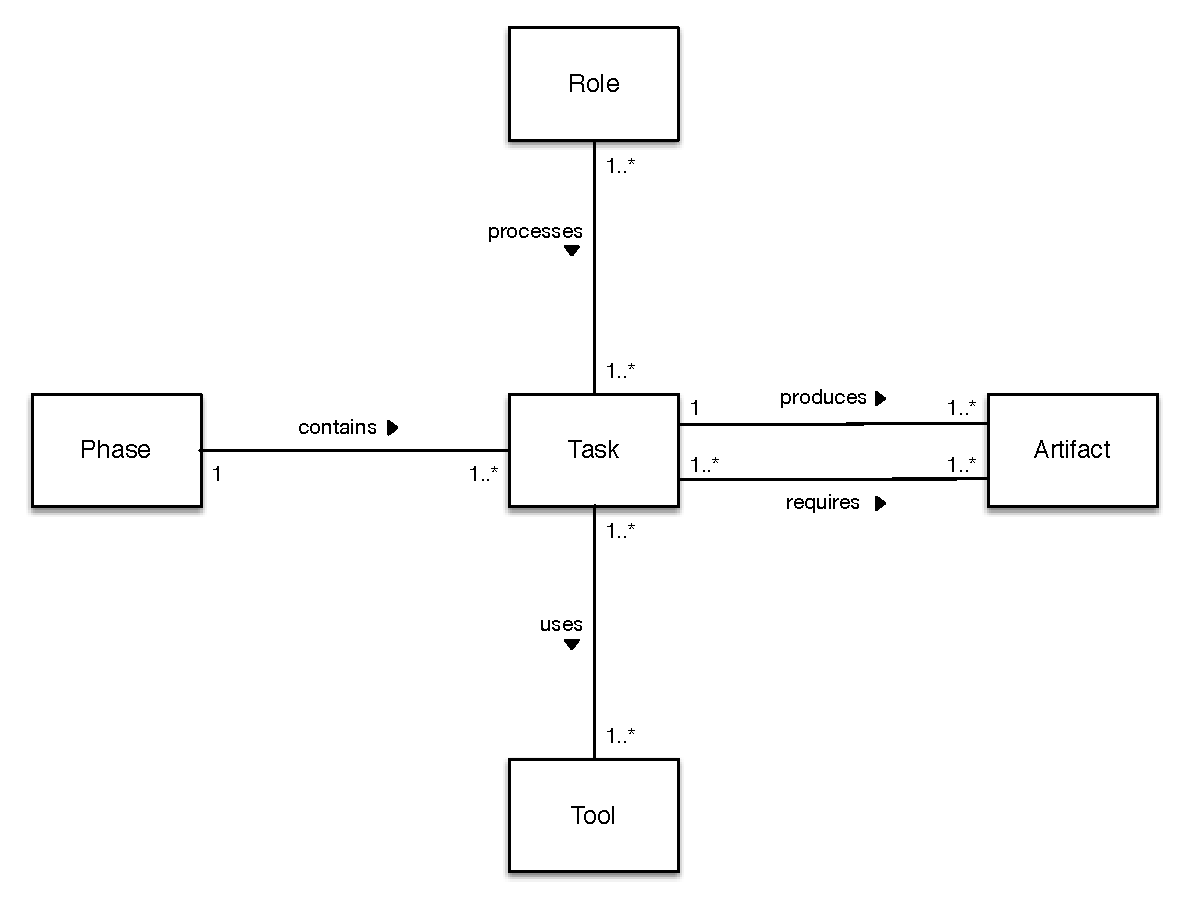
\includegraphics[width=\textwidth]{ch6_metamodel} 
	\caption{Metamodel} 
	\label{fig:ch6_metamodel} 
\end{figure}

\section{Phase}
Phases are the top-level entitis of the conceptual framework. They correspond to the different phases of the software development lifecycle and are a mean to group the different tasks of the framework.

The conceptual framework defines the following phases:
\begin{itemize}
	\item \textbf{Plan}\\
	The plan phase contains tasks relevant for the analysis and design of the system, such as the definition of the service interfaces, definition of the integration architecture and definition of performance tests.
	\item \textbf{Build}\\
	The build phase contains tasks relevant for the implementation of the system, such as the implementation of services, implementation of the integration layer and the implementation of the feedback-control subsystems.
	\item \textbf{Run}\\
	The run phase contains tasks relevant to the operation of the developed system, such as monitoring, setup and tuning.
\end{itemize}

It should be noted that the framework defines no requirements regarding the general order or mode in which theses phases and their tasks should be processed. It is therefore possible to use this framework with different software development methodologies such as the Waterfall model, Scrum or the V-Modell.

\subsection{Plan}
	\begin{tabularx}{\textwidth}{@{} l X @{}}
		\caption{Phase: Plan}\label{table:ch6_View_Plan}\\
		\toprule
		\bfseries Phase & Plan\\
		\midrule 
		\bfseries Description & This phase contains tasks concerning the technical and business design of the system.\\
		\midrule
		\bfseries Tasks & \begin{itemize}
			\item Define Service Interfaces
			\item Define Aggregation Rules
			\item Define Integration Architecture
			\item Define Routing Rules
			\item Define Controller Architecture
			\item Define Performance Tests
			\item Evaluate Test Results
			\item Perform Staffing
			\item Define Training Concept
			\item Source Project Environments
		\end{itemize}\\
		\midrule
		\bfseries Roles & \begin{itemize}
			\item Project Manager
			\item Business Analyst
			\item System Architect
			\item Test Engineer
		\end{itemize}\\
		\bottomrule
	\end{tabularx}
	
\subsection{Build}
\begin{tabularx}{\textwidth}{@{} l X @{}}
	\caption{Phase: Build}\label{table:ch6_View_Build}\\
	\toprule
	\bfseries Phase & Build\\
	\midrule 
	\bfseries Description & This phase contains tasks concerning the implementation of the system.\\
	\midrule 
	\bfseries Tasks & 
	\begin{itemize}
		\item Implement Integration Architecture
		\item Implement Service Interfaces
		\item Implement Aggregation Rules
		\item Implement Routing Rules
		\item Implement Feedback-Control	
		\item Perform Controller Tuning
	\end{itemize}
	\\
	\midrule
	\bfseries Roles & Software Engineer
	\\
	\bottomrule
\end{tabularx}


\subsection{Run}
\begin{tabularx}{\textwidth}{@{} l X @{}}
	\caption{Phase: Run}\label{table:ch6_View_Run}\\
	\toprule
	\bfseries Phase & Run\\
	\midrule 
	\bfseries Description & This phase contains tasks concerning the operation of the implemented system in the production environment. \\
	\midrule 
	\bfseries Tasks & 
	\begin{itemize}
		\item Setup Monitoring Infrastructure
		\item Setup Test Environment
		\item Perform Performance Tests
	\end{itemize}
	\\
	\midrule 
	\bfseries Roles &
	\begin{itemize}
		\item Operations Engineer
		\item Test Engineer
	\end{itemize}
	\\
	\bottomrule 
\end{tabularx}

\section{Roles}
\label{sec:ch6_roles}

Roles represent the actors, which process tasks, that is, they describe \emph{who} does something. The description of a role contains its reponsibilities and needed skills. 
A role is not the same as a person, a single person can have multiple roles and change the role according to the context of the current task.

The Conceptual Framework defines the following roles:
\begin{itemize}
	\item \textbf{Business Architect}\\
	The business architect is responsible for defining the business architecture of the software system.
	\item \textbf{System Architect}\\ 
	The system architect is responsible for defining the technical architecture of the software system.
	\item \textbf{Software Engineer}\\
	The software engineer ist responsible for implementing the software system.
	\item \textbf{Test Engineer}\\
	The test engineer is responsible for defining and performing the system test.
	\item \textbf{Operations Engineer}\\
	The operations engineer is responsible for all aspects concerned with running the developed software system.
	\item \textbf{Project Manager}\\
	The project manager is responsible for managing the software development process.
\end{itemize}

\subsection{Business Architect}

\begin{figure}[htpb] \centering 
	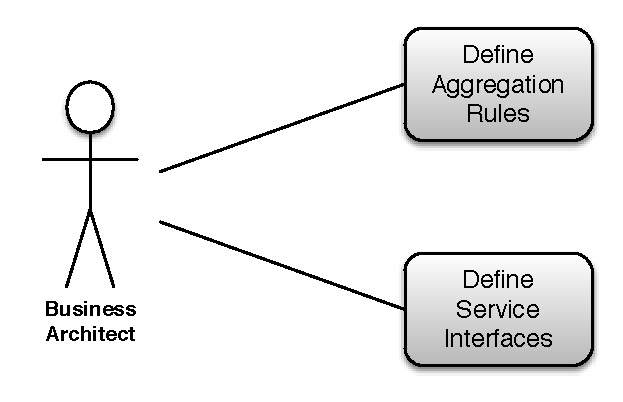
\includegraphics[width=0.5\textwidth]{ch6_role_business_architect} 
	\caption{Role: Business Architect} 
	\label{fig:ch6_role_business_architect} 
\end{figure}

\begin{tabularx}{\textwidth}{@{} l X @{}}
	\caption{Business Architect} \label{table:ch6_Role_Business_Analysist}\\
	\toprule
	\bfseries Role & Business Architect\\
	\midrule
	\bfseries Description & The Business Architect is responsible for designing the business architecture of the system, including the definition of services and aggregation rules.\\
	\midrule
	\bfseries Tasks & 
	\begin{itemize}
		\item Define Service Interfaces
		\item Define Aggregation Rules
	\end{itemize}
	\\
	\midrule 
	\bfseries Needed skills &
	\begin{itemize}
		\item Integration styles and patterns, e.g. \ac{SOA}
		\item Concepts of the Adaptive Middleware for Bulk Data Processing
		\item Business domain knowledge
	\end{itemize}
	\\
	\bottomrule
\end{tabularx}

\subsection{System Architect} 

\begin{figure}[htpb] \centering 
	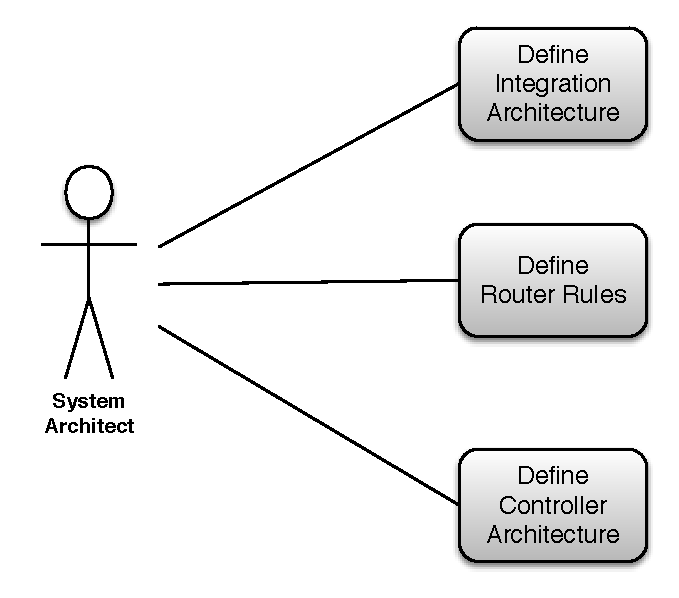
\includegraphics[width=0.5\textwidth]{ch6_role_system_architect} 
	\caption{Role: System Architect} 
	\label{fig:ch6_role_system_architect} 
\end{figure}

\newpage

\begin{tabularx}{\textwidth}{@{} l X @{}}
	\caption{System Architect}\label{table:ch6_Role_System_Architect}\\
	\toprule 
	\bfseries Role & System Architect\\
	\midrule
	\bfseries Description & The System Architect is responsible for designing the technical architecture of the system, including the integration and controller architecture.\\
	\midrule
	\bfseries Tasks & 
	\begin{itemize}
		\item Define Integration Architecture
		\item Define Controller Architecture
	\end{itemize}
	\\
	\midrule
	\bfseries Needed skills & 
	\begin{itemize}
		\item System modelling languages, e.g. \ac{UML} and tools
		\item Integration styles and patterns, e.g. \ac{SOA}
		\item Processing styles, e.g. batch and single-event processing
		\item Integration middleware technologies and products, e.g. Apache Camel, \ac{ESB}
		\item Concepts of the Adaptive Middleware for Bulk Data Processing
		\item Control theory
	\end{itemize}
	\\
	\bottomrule
\end{tabularx}


\subsection{Software Engineer}

\begin{figure}[htpb] \centering 
	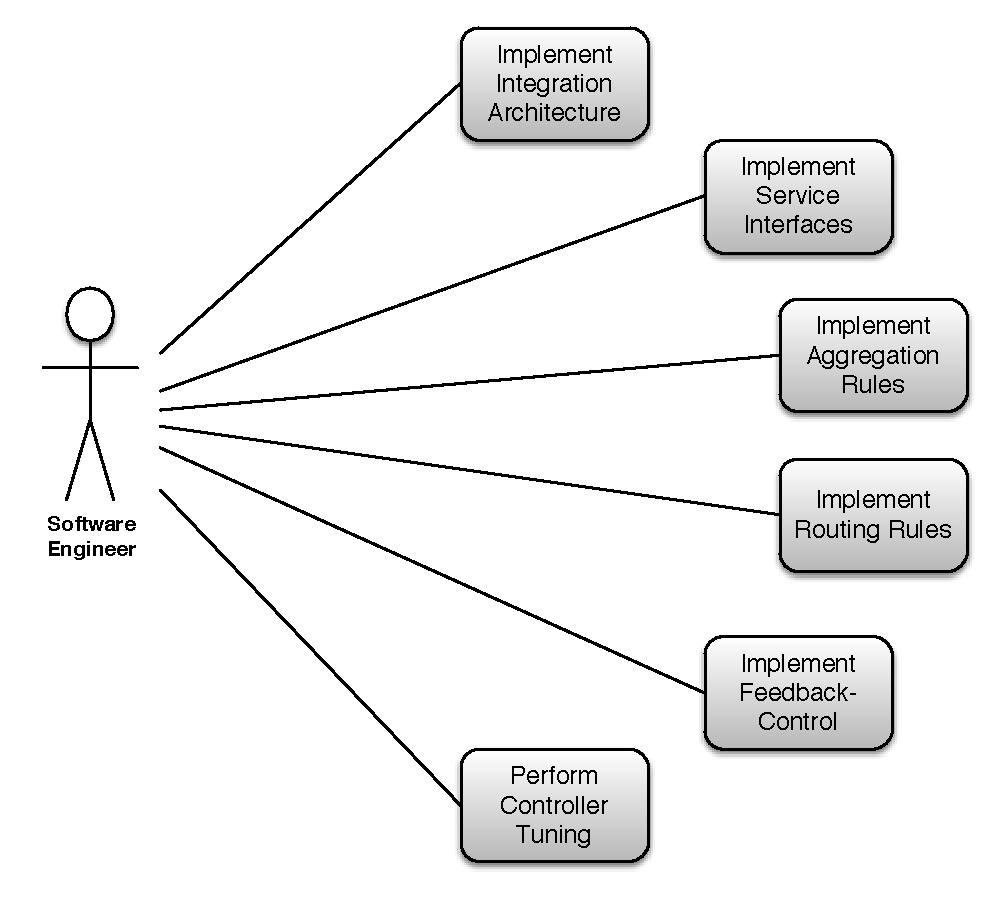
\includegraphics[width=0.5\textwidth]{ch6_role_software_engineer} 
	\caption{Role: Software Engineer} 
	\label{fig:ch6_role_software_engineer} 
\end{figure}

\begin{tabularx}{\textwidth}{@{} l X @{}}
	\caption{Software Engineer} \label{table:ch6_Role_Developer}\\
	\toprule 
	\bfseries Role & Developer\\
	\midrule
	\bfseries Description & The Developer is responsible for the implementation of the system, including the implementation and tuning of the feeback-controll loop.\\
	\midrule
	\bfseries Tasks & 
	\begin{itemize}
		\item Implement Integration Architecture
		\item Implement Service Interfaces
		\item Implement Aggregation Rules
		\item Implement Routing Rules
		\item Implement Feedback-Control
		\item Perform Controller Tuning
	\end{itemize}
	\\
	\midrule 
	\bfseries Needed skills &
	\begin{itemize}
		\item Integration styles and patterns, e.g. \ac{SOA}
		\item Processing styles, e.g. batch and single-event processing
		\item Batch optimisations
		\item Integration middleware technologies and products, e.g. Apache Camel, \ac{ESB}
		\item Concepts of the Adaptive Middleware for Bulk Data Processing
		\item Control theory
	\end{itemize}
	\\
	\bottomrule
\end{tabularx}


\subsection{Test Engineer}

\begin{figure}[htpb] \centering 
	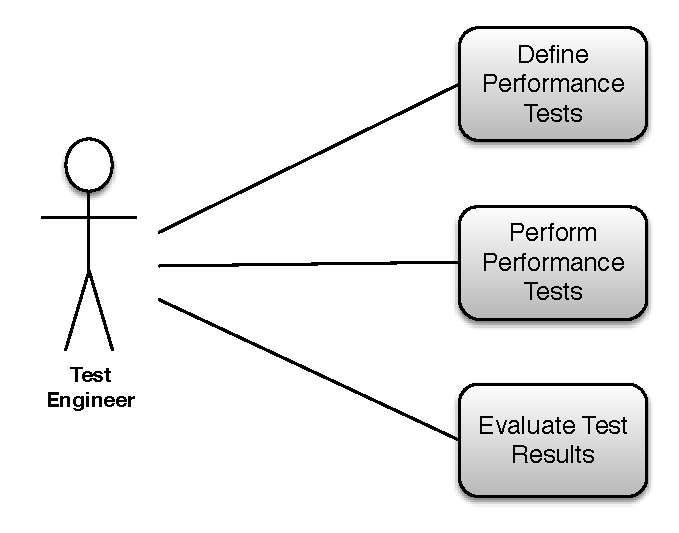
\includegraphics[width=0.5\textwidth]{ch6_role_test_engineer} 
	\caption{Role: Test Engineer} 
	\label{fig:ch6_role_test_engineer} 
\end{figure}

\begin{tabularx}{\textwidth}{@{} l X @{}}
	\caption{Test Engineer} \label{table:ch6_Role_Test_Engineer}\\
	\toprule
	\bfseries Role & Test Engineer\\
	\midrule
	\bfseries Description & The Tester is responsible for defining and performing the performance tests of the system.\\
	\midrule
	\bfseries Tasks & 
	\begin{itemize}
		\item Define Performance Tests
		\item Perform Performance Tests
		\item Evaluate Performance Tests
	\end{itemize}
	\\
	\midrule
	\bfseries Needed skills &
	\begin{itemize}
		\item Design and evaluation of performance tests
		\item Concepts of the Adaptive Middleware for Bulk Data Processing
		\item Control theory (basics)
	\end{itemize}
	\\
	\bottomrule
\end{tabularx}


\subsection{Operations Engineer}
\begin{figure}[htpb] \centering 
	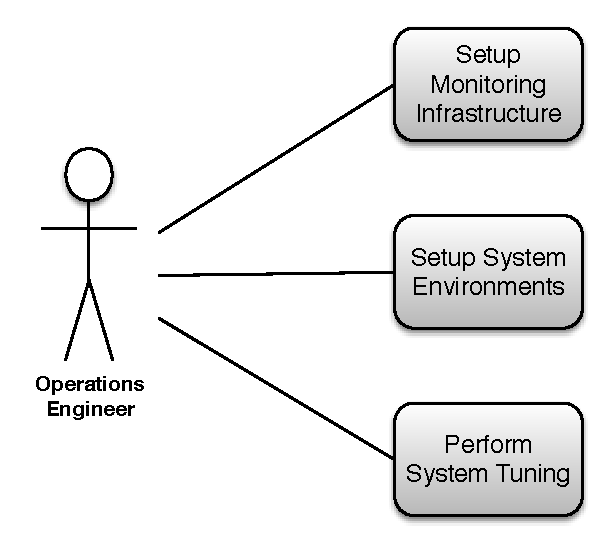
\includegraphics[width=0.5\textwidth]{ch6_role_operations_engineer} 
	\caption{Role: Operations Engineer} 
	\label{fig:ch6_role_operations_engineer} 
\end{figure}

\begin{tabularx}{\textwidth}{@{} l X @{}}
	\caption{Operations Engineer}\label{table:ch6_Role_Operations_Engineer}\\
	\toprule
	\bfseries Role & Operations Engineer\\
	\midrule
	\bfseries Description & The Operations Engineer is responsible for operating the system, including setup, deployment and monitoring.\\
	\midrule
	\bfseries Tasks & 
	\begin{itemize}
		\item Setup Monitoring Infrastructure
		\item Setup System Environments
		\item Perform System Tuning
	\end{itemize}
	\\
	\midrule
	\bfseries Needed skills &
	\begin{itemize}
		\item Monitoring technologies and products, e.g. \ac{JMX}
		\item Concepts of the Adaptive Middleware for Bulk Data Processing
	\end{itemize}
	\\
	\endline
\end{tabularx}

\newpage

\subsection{Project Manager}

\begin{figure}[htpb] \centering 
	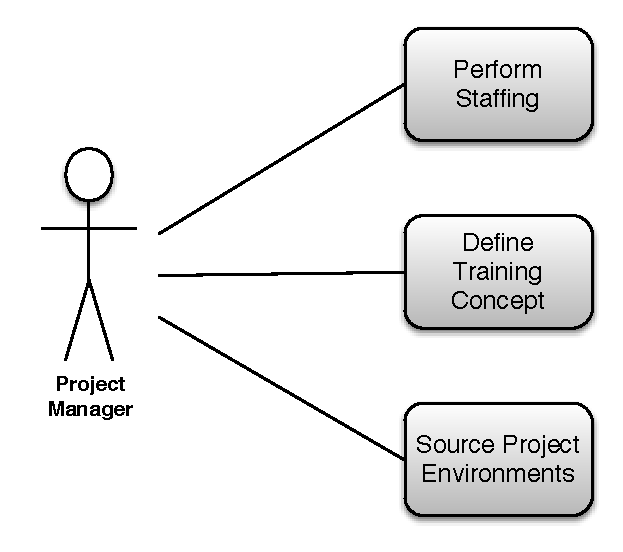
\includegraphics[width=0.5\textwidth]{ch6_role_project_manager} 
	\caption{Role: Project Manager} 
	\label{fig:ch6_role_project_manager} 
\end{figure}

\begin{tabularx}{\textwidth}{@{} l X @{}}
	\caption{table}{Project Manager} \label{table:ch6_Role_Project_Manager}\\
	\toprule
	\bfseries Role & Project Manager\\
	\midrule
	\bfseries Description & The Project Manager is responsible for the project coordination, including the staffing and planing of the required environments.\\
	\midrule
	\bfseries Tasks & 
	\begin{itemize}
		\item Perform Staffing
		\item Define Training Concept
		\item Source Project Environments
	\end{itemize}
	\\
	\midrule 
	\bfseries Needed skills &
	\begin{itemize}
		\item Framework for Feedback-Controlled Bulk Data Processing Systems
		\item Concepts of the Adaptive Middleware for Bulk Data Processing
	\end{itemize}
	\\
	\bottomrule
\end{tabularx}


\section{Tasks}
\label{sec:ch6_tasks}

Tasks are the main entities of the conceptual framework. A Tasks describes \emph{what} should be done, \emph{why} should it be done, and \emph{who} should do it.
Additionally, it describes the required and produced artifacts, the tools that should be used to process the task and the expected challenges.

Tasks depend on each other, some tasks must be processed in a certain order. A task can have multiple subtasks.

The Conceptual Framework only describes tasks that are specific to the design and implementation of an Adaptive Middleware for Bulk Data Processing as described in chapter \ref{ch:adaptive_middleware}. It does not describe common tasks or activities that are needed for every software system.

Figure \ref{fig:ch6_overview_tasks} shows an overview of the tasks grouped by the different phases of the Conceptual Framework.

\begin{figure}[htpb] \centering 
	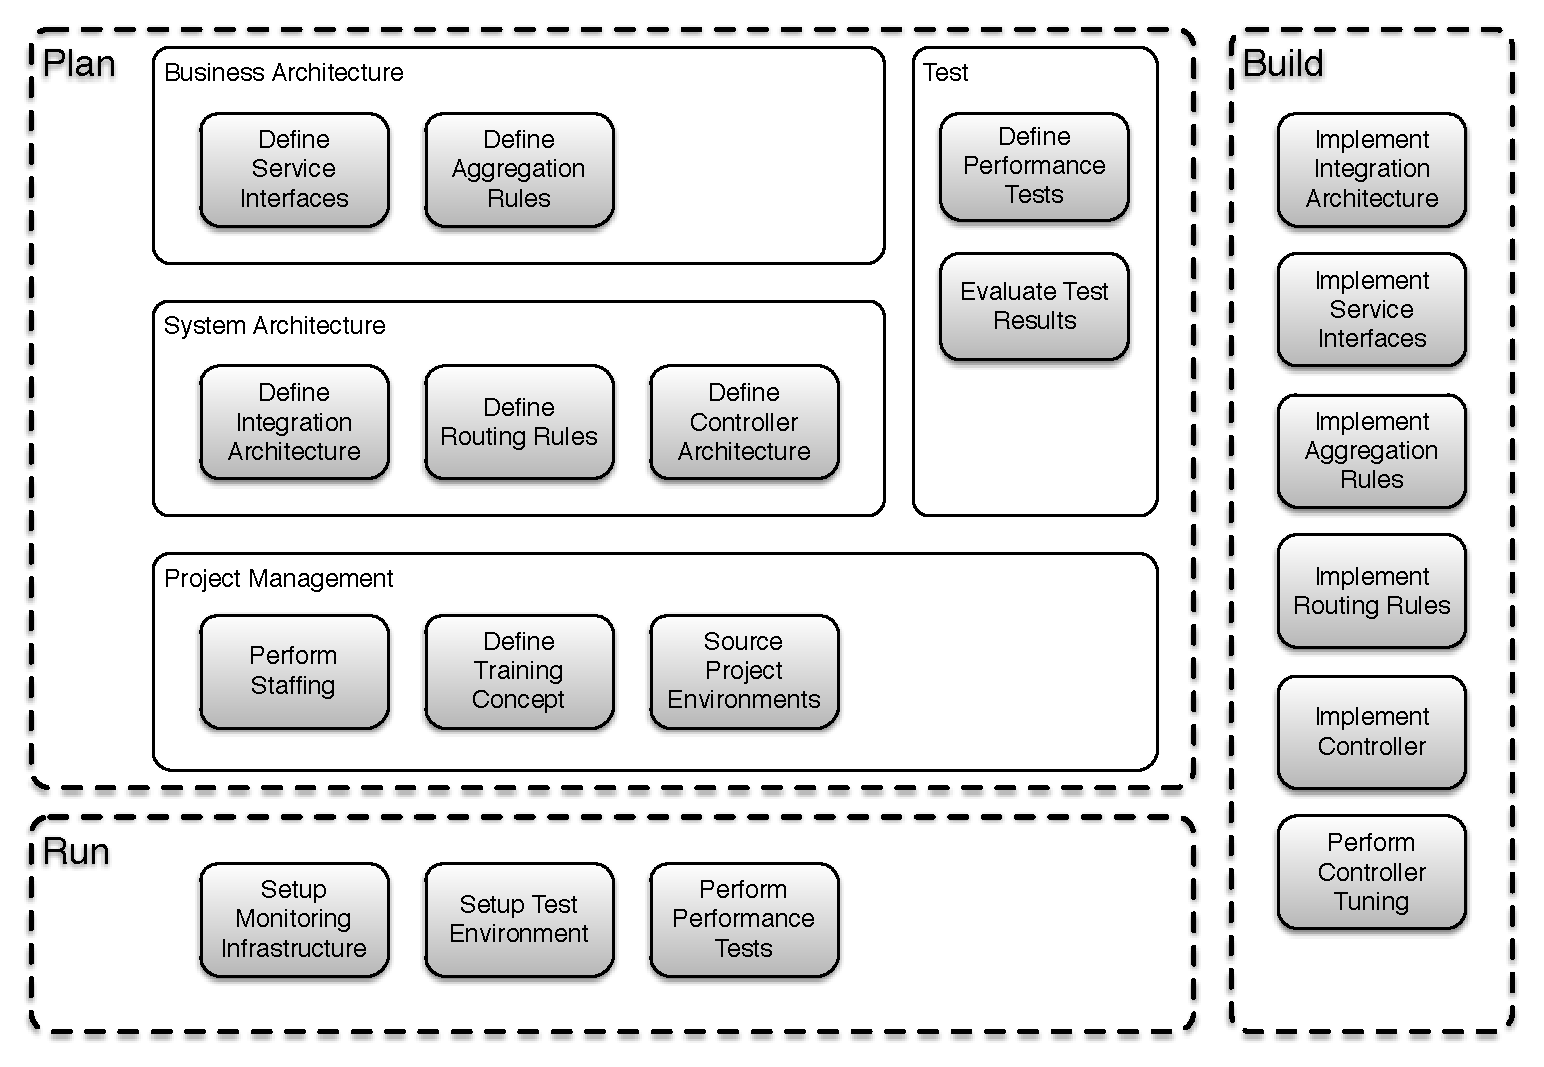
\includegraphics[width=\textwidth]{ch6_overview_tasks} 
	\caption{Overview of tasks} 
	\label{fig:ch6_overview_tasks} 
\end{figure}

The following tasks are defined:

\begin{itemize}
	\item Business Architecture
	\begin{itemize}
		\item Define Performance Requirements
		\item Define Service Interfaces
		\item Define Aggregation Rules
	\end{itemize}
	\item System Architecture 
	\begin{itemize}
		\item Define Integration Architecture
		\item Define Routing Rules
		\item Define Controller Architecture 
		\begin{itemize}
			\item Define Control Problem 
			\item Define Input/Output Variables 
		\end{itemize}
		\item Define Routing Rules
	\end{itemize}
	\item Implementation
	\begin{itemize}
		\item Implement Controller / Feedback Loop
		\item Perform Controller Tuning 
		\begin{itemize}
			\item System Model/System Identification 
			\item Static Tests
			\item Step Tests
		\end{itemize}
		\item Implement Integration Architecture
		\item Implement Service Interfaces
		\item Implement Aggregation Rules 
		\item Implement Routing Rules
	\end{itemize}
	\item Test
	\begin{itemize}
		\item Define Performance Tests 
		\item Evaluate Performance Test Results
	\end{itemize}
	\item Operation
	\begin{itemize}
		\item Setup Monitoring infrastructure
		\item Setup Test and Integration Environment
		\item Perform Performance Tests
	\end{itemize} 
	\item Project Management
	\begin{itemize}
		\item Define Training Concept
		\item Staffing
	\end{itemize}
\end{itemize}

\subsection{Business Architecture}

The business architecture defines the business components of the system and their relationships independantly of the technical implementation.
Except from the described subtasks, the task is not specific to the conceptual model.

\begin{figure}[htpb] \centering 
	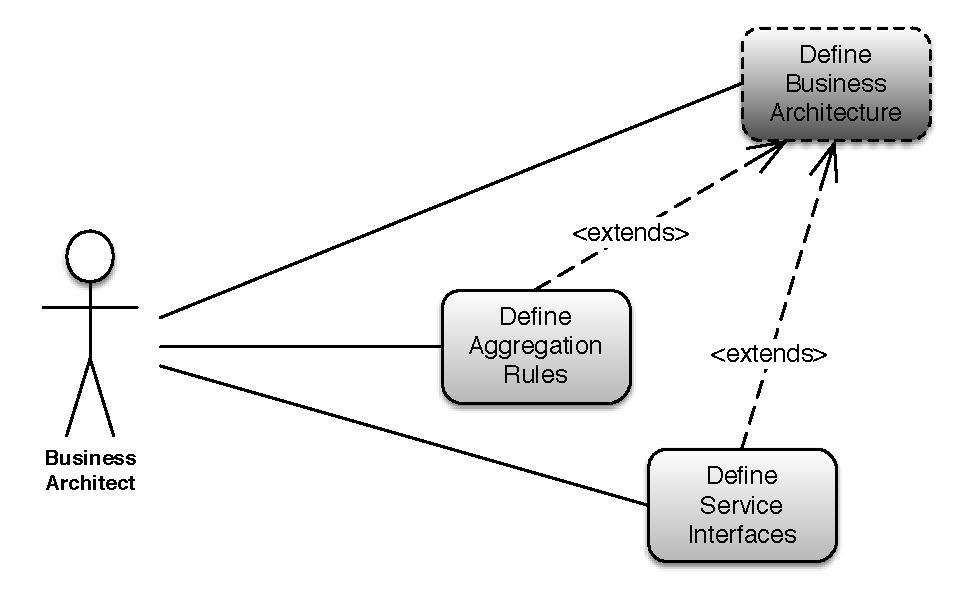
\includegraphics[width=\textwidth]{ch6_tasks_business_architecture} 
	\caption{Tasks extending the definition of the business architecture} 
	\label{fig:ch6_tasks_business_architecture} 
\end{figure}

\subsubsection{Define Performance Requirements}
\begin{tabularx}{\textwidth}{@{} l X @{}}
	\caption{Define Performance Requirements} \label{table:ch6_Task_Define_Performance Requirements}\\
	\toprule
	\bfseries Task & Define Performance Requirements\\
	\midrule\bfseries What & 
	\begin{itemize}
		\item Definition of workload scenarios
		\item Definition of requirements regarding throughput and latency of the system
		\begin{itemize}
			\item What is the required minimal latency of the system?
			\item What is the required minimal throughput of the system?
		\end{itemize}
	\end{itemize}
	\\
	\midrule
	\bfseries Why &
	\begin{itemize}
		\item The performance requirements are needed for the desing of the system architecture
	\end{itemize}\\
	\midrule
	\bfseries Who & 
	\begin{itemize}
		\item Busines Analyst
		\item System Architect
	\end{itemize}\\
	\midrule
	\bfseries Output & Performance Requirements\\
	\midrule
	\bfseries Challenges & The performance requirements must be explicitely defined in a way that they can be evaluated.\\
	\bottomrule
\end{tabularx}

\subsubsection{Define Service Interfaces}
\begin{tabularx}{\textwidth}{@{} l X @{}}
	\caption{Define Service Interfaces} \label{table:ch6_Task_Define_Service_Interfaces}\\
	\toprule
	\bfseries Task & Define Service Interfaces\\
	\midrule\bfseries What & 
	\begin{itemize}
		\item Structuring the functionality of the system into business services
		\item Services may already exist or need to be implemented.
		\item Definition of needed services and their operations, every service needs operations for single event and batch processing
		\begin{itemize}
			\item Distinct operations for batch and single event processing
			\item common operation for both processing styles (list interface)
		\end{itemize}
		\item Defines the structure of input and output data
		\item Does not include informations about the technical format, such as \ac{XML} or \ac{JSON}, and the integration style, such SOAP or \ac{REST}
	\end{itemize}
	\\
	\midrule
	\bfseries Why &
	\begin{itemize}
		\item Defines the business components (services) of the system
		\item Basis for the definition of the integration architecture and the implementation of the services.
	\end{itemize}\\
	\midrule
	\bfseries Who & Business Architect\\
	\midrule
	\bfseries Output & Service Interface Definitions\\
	\midrule
	\bfseries Challenges & Finding the appropriate services and service granularity\\
	\bottomrule
\end{tabularx}

\subsubsection{Define Aggregation Rules}
\begin{tabularx}{\textwidth}{@{} l X @{}}
	\caption{Define Aggregation Rules} \label{table:ch6_Task_Define_Aggregation_Rules}\\
	\toprule
	\bfseries Task & Define Aggregation Rules\\
	\midrule
	\bfseries What & 
	\begin{itemize}
		\item Definition of rules used in the aggregator for correlating events
		\item Different options
		\begin{itemize}
			\item No correlation
			\begin{itemize}
				\item Simple solution
				\item even distribution of events
				\item optimization is not or hardly possible
			\end{itemize}
			\item Business correlation
			\begin{itemize}
				\item analysation of processed data needed
				\item no even distribution of data (depending on correlation rule), leads to uneven distribution of latency
				\item optimization is possible
			\end{itemize}
			\item Technical correlation
			\begin{itemize}
				\item analysation of processed data needed
				\item Rules can be defined after integration architecture
				\item no even distribution of data (depending on correlation rule), leads to uneven distribution of latency
				\item optimization is possible
			\end{itemize}
		\end{itemize}
	\end{itemize}
	\\
	\midrule
	\bfseries Why & The aggregation Rules are needed by the Aggregator to correlate events.\\
	\midrule
	\bfseries Who & 
	\begin{itemize}
		\item Business Architect
		\item System Architect
	\end{itemize}
	\\
	\midrule
	\bfseries Output & Aggregation Rules\\
	\midrule
	\bfseries Challenges & 
	\begin{itemize}
		\item Finding aggregation rules that allows for an even distribution of events.
		\item Technical Aggregation Rules can be defined only after the definition of the integration architecture
	\end{itemize}\\
	\bottomrule 
\end{tabularx}

\subsection{System Architecture}

The system architecture defines the technical architecture of the system. Except from the described subtasks, the task is not specific to the conceptual model.

\begin{figure}[htpb] \centering 
	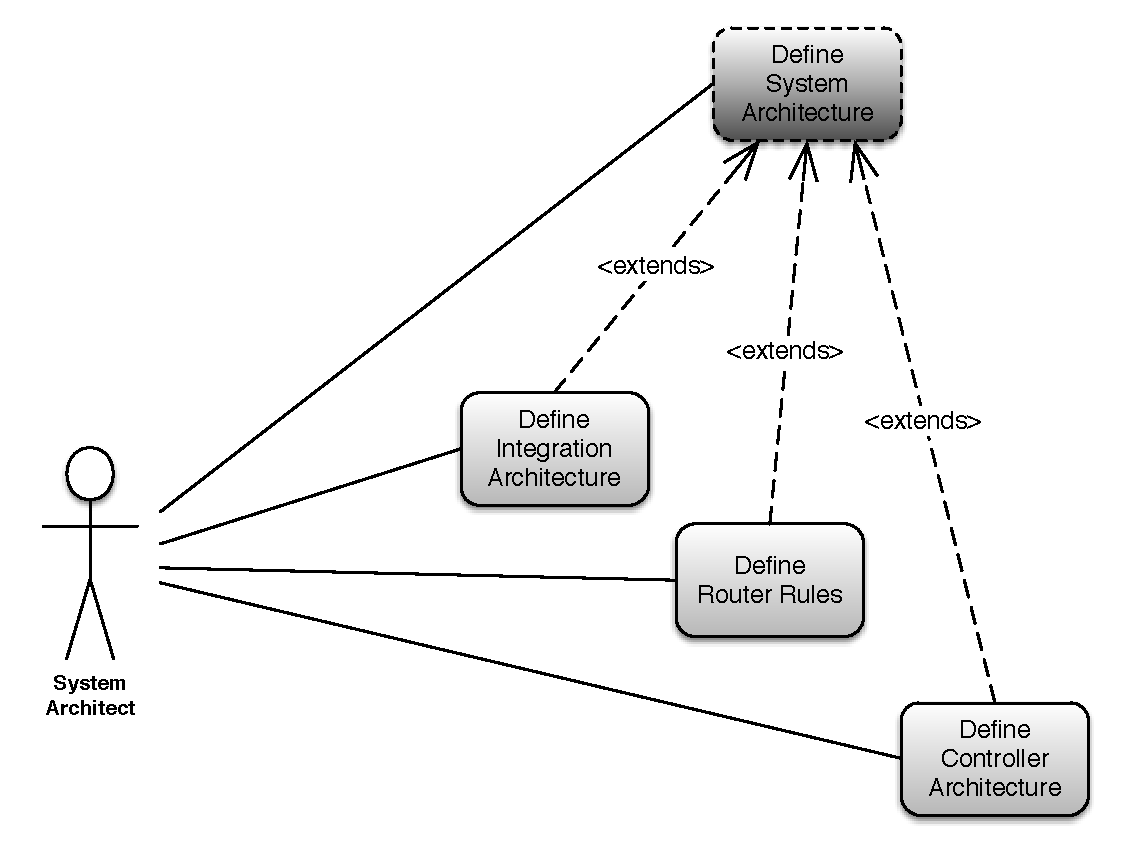
\includegraphics[width=\textwidth]{ch6_tasks_system_architecture} 
	\caption{Tasks extending the definition of the system architecture} 
	\label{fig:ch6_tasks_system_architecture} 
\end{figure}

\subsubsection{Define Integration Architecture}
\begin{tabularx}{\textwidth}{@{} l X @{}}
	\caption{Define Integration Architecture} \label{table:ch6_Task_Define_Integration_Architecture}\\
	\toprule
	\bfseries Task & Define Integration Architecture\\
	\midrule
	\bfseries What &
	\begin{itemize}
		\item Definition of integration architecture
		\begin{itemize}
			\item Sychronous, e.g. webservices
			\item Asynchronous, e.g. message queues
		\end{itemize}
		\item Choosing a middleware technology or product
		\item Definition of transports
		\begin{itemize}
			\item JMS
			\item SOAP
			\item REST
			\item FTP
			\item DB
		\end{itemize}
		\item Different transports / integration patterns needed for different aggregation sizes:
		\begin{itemize}
			\item Large messages should not be transferred over the messaging bus
			\item Options for large messages:
			\begin{itemize}
				\item File-based integration and transfer using FTP or database
				\item Message-Slip EIP pattern
			\end{itemize}
		\end{itemize}
	\end{itemize}
	\\
	\midrule
	\bfseries Why & The integration architecture defines the technologies to integrate the services into the system.\\
	\midrule
	\bfseries Who & System Architect\\
	\midrule 
	\bfseries Input & Service Interface Definitions
	\\
	\midrule 
	\bfseries Output & Integration Architecture\\
	\midrule
	\bfseries Challenges & Choosing the appropriate middleware technology and or product.\\
	\bottomrule
\end{tabularx}

\subsubsection{Define Routing Rules}
\begin{tabularx}{\textwidth}{@{} l X @{}}
	\caption{table}{Define Routing Rules} \label{table:ch6_Task_Define_Routing_Rules}\\
	\toprule 
	\bfseries Task & Define Routing Rules\\
	\midrule 
	\bfseries What & 
	\begin{itemize}
		\item Depending on the size of the aggregated message, the Router routes the message to the appropriate service endpoint, which is either optimized for batch or single event processing.
		\item The routing rules define, which service endpoint should be called for a given aggregation size.
	\end{itemize}
	\\
	\midrule 
	\bfseries Why & The routing rules define, which service endpoint should be called for a given aggregation size.\\
	\midrule
	\bfseries Who & System Architect\\
	\midrule
	\bfseries Input & Integration Architecture
	\\
	\midrule 
	\bfseries Output & Routing Rules Definition\\
	\midrule 
	\bfseries Challenges & Finding the data aggregation threshold to route messages to the appropriate service endpoint.\\
	\bottomrule 
\end{tabularx}

\subsubsection{Define Controller Architecture}

\begin{tabularx}{\textwidth}{@{} l X @{}}
	\caption{Define Controller Architecture} \label{table:ch6_Task_Define_Controller_Architecture}\\
	\toprule 
	\bfseries Task & Define Controller Architecture\\
	\midrule 
	\bfseries What & 
	\begin{itemize}
		\item Design of the controller architecture implemented by the system
		\item For example
		\begin{itemize}
			\item PID Controller
			\item Fuzzy Controller
		\end{itemize}
		\item Depends on control problem and system dynamics (linear, non-linear)
	\end{itemize}
	\\
	\midrule 
	\bfseries Why & The Controller Architecture is the basis for the implementation of the feedback-control loop.\\
	\midrule 
	\bfseries Who & System Architect\\
	\midrule 
	\bfseries Input & Integration Architecture\\
	\midrule 
	\bfseries Output & Controller Architecture\\
	\midrule 
	\bfseries Challenges & Finding the right controller architecture is an iterative process. A simple solution should be used initially, which should be refined when the system is implemented. Alternatively, a simulation can be used to evaluate the controller architecture beforehand.\\
	\bottomrule 
\end{tabularx}

\subsubsection{Define Control Problem}

\begin{tabularx}{\textwidth}{@{} l X @{}}
	\caption{Define Control Problem} \label{table:ch6_Task_Define_Control_Problem}\\
	\toprule 
	\bfseries Task & Define Control Problem\\
	\midrule 
	\bfseries What & 
	\begin{itemize}
		\item Define what properties of the system should be controlled.
		\item In case of the Adaptive Middleware (see Chapter \ref{ch:adaptive_middleware}) the control problem is already defined.
	\end{itemize}
	\\
	\midrule 
	\bfseries Why & The control problem defines the goal of the feedback-control.\\
	\midrule 
	\bfseries Who & System Architect\\
	\midrule 
	\bfseries Output & Control Problem\\
	\midrule 
	\bfseries Challenges & \\
	\bottomrule 
\end{tabularx}


\subsubsection{Define Input/Output Variables}

\begin{tabularx}{\textwidth}{@{} l X @{}}
	\caption{Define Input/Output Variables} \label{table:ch6_Task_Define_Controller_Variables}\\
	\toprule 
	\bfseries Task & Define Input/Output Variables\\
	\midrule 
	\bfseries What &
	\begin{itemize}
		\item Definition of input and output variables of the controller
		\item for example
		\begin{itemize}
			\item Number of messages in the system
			\item Input queue length
			\item Current end-to-end latency
			\item Current throughput
		\end{itemize}
	\end{itemize}
	\\
	\midrule 
	\bfseries Why & The input/output variables are needed for the implementation of the controller.\\
	\midrule 
	\bfseries Who & System Architect\\
	\midrule 
	\bfseries Input & Control Problem\\
	\midrule 
	\bfseries Output & Input/Output Variables\\
	\midrule 
	\bfseries Challenges & The selected input variables should be measured easily and directly, without delay such as when calculating averages.\\
	\bottomrule 
\end{tabularx}

\subsection{Implementation}

\subsubsection{Implement Controller}

\begin{tabularx}{\textwidth}{@{} l X @{}}
	\caption{Implement Controller / Feedback Loop} \label{table:ch6_Task_Implement_Controller}\\
	\toprule 
	\bfseries Task & Implement Feedback-Control Loop\\
	\midrule 
	\bfseries What & 
	\begin{itemize}
		\item Implementation of Controller Architecture including
		\begin{itemize}
			\item Sensors
			\item Controller
			\item Actuator
		\end{itemize}
		\item Implement JMX Beans for monitoring purposes
		\item Implement mechanisms for performing static and step tests.
	\end{itemize}
	\\
	\midrule 
	\bfseries Why & The Feedback-Control Loop implements the automatic adjustment of data granularity at runtime.\\
	\midrule 
	\bfseries Who & Software Engineer\\
	\midrule 
	\bfseries Input & Controller Architecture\\
	\midrule 
	\bfseries Challenges & 
		\begin{itemize}
			\item Sensor performance
			\item Distributed sensors 
			\item Framework vs. custom development
		\end{itemize}\\
	\bottomrule 
\end{tabularx}


\subsubsection{Static Tests}

\begin{tabularx}{\textwidth}{@{} l X @{}}
	\caption{Static Tests} \label{table:ch6_Task_Static_Tests}\\
	\toprule 
	\bfseries Task & Static Tests\\
	\midrule 
	\bfseries What & Perform static tests in order to determine the static behaviour of the system.\\
	\midrule 
	\bfseries Why & The static behaviour of the system is needed to determine the characteristics of the system.\\
	\midrule 
	\bfseries Who & System Architect\\
	\midrule 
	\bfseries Output & Static Test Results\\
	\midrule 
	\bfseries Tools & 
	\begin{itemize}
		\item Tools for data processing
		\item Tools for data visualisation
	\end{itemize}\\
	\midrule
	\bfseries Challenges & The system needs to be already implemented. Alternatively, an appropriate model of the system can be used.
	\\
	\bottomrule
\end{tabularx}


\subsubsection{Step Tests}

\begin{tabularx}{\textwidth}{@{} l X @{}}
	\caption{Step Tests} \label{table:ch6_Task_Step_Tests}\\
	\toprule 
	\bfseries Task & Step Tests\\
	\midrule 
	\bfseries What & Perform step tests to determine the dynamic behaviour of the system.\\
	\midrule 
	\bfseries Why & The dynamic behaviour of the system is needed for building a model of the system and to tune the controller.\\
	\midrule 
	\bfseries Who & System Architect\\
	\midrule 
	\bfseries Output & Step Test Results\\
	\midrule 
	\bfseries Tools & 
	\begin{itemize}
		\item Tools for data processing
		\item Tools for data visualisation
	\end{itemize}\\
	\midrule
	\bfseries Challenges & The system needs to be already implemented. Alternatively, an appropriate model of the system can be used.
	\\
	\bottomrule 
\end{tabularx}


\subsubsection{System Model/System Identification}
	\begin{tabularx}{\textwidth}{@{} l X @{}}
		\caption{System Model/System Identification} \label{table:ch6_Task_Controler_Tuning}\\
		\toprule 
		\bfseries Task & Define System Architecture\\
		\midrule 
		\bfseries What & Building a model of the system.\\
		\midrule 
		\bfseries Why & The system model is used to build a simulation of the system which can be used for implementing the controller.\\
		\midrule 
		\bfseries Who & System Architect\\
		\midrule 
		\bfseries Input & Static and dynamic behaviour of the system\\ 
		\midrule 
		\bfseries Output & System Model\\
		\midrule 
		\bfseries Tools & Tools for system modelling and system identification \\
		\midrule 
		\bfseries Challenges & The software engineer needs to have a profound knowlegde of controller theory and system identification in order to build a relevant model of the system.
			\\
		\bottomrule 
	\end{tabularx}

\subsubsection{Perform Controller Tuning}
	\begin{tabularx}{\textwidth}{@{} l X @{}}
		\caption{Perform Controller Tuning} \label{table:ch6_Task_Perform_Controller_Tuning} \\
		\toprule 
		\bfseries Task & Perform Controller Tuning\\
		\midrule 
		\bfseries What & 
		\begin{itemize}
			\item Controller Tuning can be done using the implementation of the system.
			\item Alternatively, the tuning can done using a model of the system.
		\end{itemize}
		\\
		\midrule 
		\bfseries Why & The Controller needs to be adjusted to the system characteristics.\\
		\midrule 
		\bfseries Who & Software Engineer\\
		\midrule 
		\bfseries Input & Controller Architecture\\
		\midrule 
		\bfseries Output & Controler Configuration\\
		\midrule
		\bfseries Tools & Tools for Simulation\\
		\midrule 
		\bfseries Challenges & The software engineer needs to have a profound knowlegde of controller theory and the controller architecture in order to properly tune the implemented controller.
		\\
		\bottomrule 
	\end{tabularx}


\subsubsection{Implement Service Interfaces}

\begin{tabularx}{\textwidth}{@{} l X @{}}
	\caption{Implement Service Interfaces} \label{table:ch6_Task_Implement_Service_Interfaces}\\
	\toprule 
	\bfseries Task & Implement Service Interfaces\\
	\midrule 
	\bfseries What & 
	\begin{itemize}
		\item Implementation of business services
		\item Batch implementation / single event implementation
		\item Batch optimisation
	\end{itemize}
	\\
	\midrule 
	\bfseries Why & The services implement the business functionality of the system.\\
	\midrule 
	\bfseries Who & Software Engineer\\
	\midrule 
	\bfseries Input & Service Interface Definitions\\
	\midrule 
	\bfseries Challenges & Implementing appropriate optimisations for batch and single-event processing.
	\\
	\bottomrule 
\end{tabularx}


\subsubsection{Implement Aggregator}
\begin{tabularx}{\textwidth}{@{} l X @{}}
	\caption{Implement Aggregator} \label{table:ch6_Task_Implement_Aggregator}\\
	\toprule 
	\bfseries Task & Implement Aggregatator\\
	\midrule 
	\bfseries What & 
	\begin{itemize}
		\item Implementation or configuration of the Aggregator component.
		\item Implementation of the aggregation rules.
		\item Rules should be configurable during run-time or configuration-time. Should not be hard-coded.
	\end{itemize}
	\\
	\midrule 
	\bfseries Why & The aggregator component is responsible for aggregating events according to the aggregation rules and is one of the main building blocks of the Adaptive Middleware (see Chapter \ref{ch:adaptive_middleware}).\\
	\midrule 
	\bfseries Who & Software Engineer\\
	\midrule 
	\bfseries Input & Aggregation Rules\\
	\midrule 
	\bfseries Challenges & Implementation of mechanisms to dynamically load aggregation rules at run-time or configuration-time.\\
	\bottomrule 
\end{tabularx}

\subsection{Test}

\subsubsection{Define Performance Tests}
\begin{tabularx}{\textwidth}{@{} l X @{}}
	\caption{Define Performance Tests} \label{table:ch6_Task_Define_Performance_Tests}\\
	\toprule 
	\bfseries Task & Define Performance Tests\\
	\midrule 
	\bfseries What &
	\begin{itemize}
		\item Define load scenarios
		\item Define test data
		\item Implement event generator
		\item Implement tools and scripts for evaluation and data visualisation
	\end{itemize}
	\\
	\midrule 
	\bfseries Why & The Performance Test Concept defines what should be done to test whether the system meets its performance requirements.\\
	\midrule 
	\bfseries Who & Test Engineer\\
	\midrule 
	\bfseries Output & Performance Test Concept\\
	\midrule
	\bfseries Tools & 
	\begin{itemize}
		\item Tools for data processing 
		\item Tools for data visualisation
	\end{itemize}\\
	\midrule
	\bfseries Challenges & The performance test should include tests concerning the adaptive behaviour of the system.\\
	\bottomrule 
\end{tabularx}

\subsubsection{Evaluate Performance Test Results}

\begin{tabularx}{\textwidth}{@{} l X @{}}
	\caption{Evaluate Performance Test Results} \label{table:ch6_Evaluate_Performance_Results}\\
	\toprule 
	\bfseries Task & Evaluate Performance Test Results\\
	\midrule 
	\bfseries What & 
	\begin{itemize}
		\item Visualise the test results using the tools/skripts implemented in the task Define Performance Tests.
	\end{itemize}
	\\
	\midrule 
	\bfseries Why & The performance test evaluation is conducted to understand the performance characteristics of the system.\\
	\midrule 
	\bfseries Who & 
	\begin{itemize}
		\item Test Engineer
		\item System Engineer
	\end{itemize}
	\\
	\midrule 
	\bfseries Input & Performance Test Result\\
	\midrule 
	\bfseries Output & Performance Test Evaluation\\
	\midrule 
	\bfseries Tools & 
	\begin{itemize}
		\item Tools for data processing
		\item Tools for data visualisation
	\end{itemize}
	\\
	\bottomrule 
\end{tabularx}

\subsection{Operations}

\subsubsection{Setup Monitoring infrastructure}
\begin{tabularx}{\textwidth}{@{} l X @{}}
	\caption{Setup Monitoring infrastructure} \label{table:ch6_Task_Setup_Monitoring_infrastructure}\\
	\toprule 
	\bfseries Task & Setup Monitoring infrastructuree\\
	\midrule 
	\bfseries What & Setting up the monitoring infrastructure, including
	\begin{itemize}
		\item Integrating the monitoring facilities (for example \ac{JMX} Beans) of the system into the existing monitoring infrastructure.
	\end{itemize}
	\\
	\midrule 
	\bfseries Why & The monitoring infrastructure is needed to monitor the system at run-time. Based on the monitoring the operation engineer is able to further tune the system.\\
	\midrule 
	\bfseries Who & Operations Engineer\\
	\midrule 
	\bfseries Input & System Architecture\\
	\midrule 
	\bfseries Challenges & \\
	\bottomrule 
\end{tabularx}

\subsubsection{Setup Test Environment}
\begin{tabularx}{\textwidth}{@{} l X @{}}
	\caption{Setup Test Environment} \label{table:ch6_Task_Setup_Test_Environment}\\
	\toprule \bfseries Task & Setup Test Environment\\
	\midrule 
	\bfseries What & Setup up the test environment used for the performance tests, including
	\begin{itemize}
		\item Setup / Mock external Services
		\item setup test data
		\item Deployment
	\end{itemize}
	\\
	\midrule 
	\bfseries Why & The test environment is needed to perform the performance tests.\\
	\midrule 
	\bfseries Who & Operations Engineer\\
	\midrule 
	\bfseries Input & Performance Test Concept\\
	\midrule 
	\bfseries Challenges & 
	\begin{itemize}
		\item The test environment should be comparable to the production environment to get valid test results.
		\item Additionally, the test data should also be comparable to production data.
	\end{itemize}
	\\
	\bottomrule
\end{tabularx}


\subsubsection{Perform Performance Tests}
\begin{tabularx}{\textwidth}{@{} l X @{}}
	\caption{Perform Performance Tests} \label{table:ch6_Task_Perform_Performance_Tests}\\
	\toprule 
	\bfseries Task & Perform Performance Tests\\
	\midrule 
	\bfseries What & \\
	\midrule 
	\bfseries Why & The performance tests are necessary to assure that the system meets the performance requirements.\\
	\midrule 
	\bfseries Who & Tesst Engineer\\
	\midrule 
	\bfseries Input & Performance Test Concept\\
	\midrule 
	\bfseries Output & Performance Test Results\\
	\midrule 
	\bfseries Challenges & To ensure the reliability of the performance test results, the tests should be run multiple times. This is often difficult with regard of the needed ressources for the performance test, such as availability of external systems.\\
	\bottomrule 
\end{tabularx}

\subsection{Project Management}

\subsubsection{Define Training Concept}

\begin{tabularx}{\textwidth}{@{} l X @{}}
	\caption{Define Training Concept} \label{table:ch6_Task_Define_Training_Concept}\\
	\toprule 
	\bfseries Task & Define Training Concept\\
	\midrule 
	\bfseries What & 
	\begin{itemize}
		\item define target audience, e.g. operations engineer
		\item define training content
		\begin{itemize}
			\item Different operation modes (batch, single event processing)
			\item performance characteristics (regarding latency and throughput) depend on current operation mode
			\item Tuning options (Controller, Aggregation Rules, Routing Rules)
		\end{itemize}
	\end{itemize}
	\\
	\midrule 
	\bfseries Why & 
	\begin{itemize}
		\item The operation engineers need to have the knowlegde to operate and tune the system in production.
		\item Additionally, the team members also need to have the knowlegde to design and implement the system.
	\end{itemize}
	\\
	\midrule 
	\bfseries Who & System Architect\\
	\midrule 
	\bfseries Input & System Architecture\\
	\midrule
	\bfseries Output & Training Concept\\
	\midrule 
	\bfseries Challenges & The training concept should consider the respective audience and its existing knowlegde.\\
	\bottomrule 
\end{tabularx}


\subsubsection{Staffing}

\begin{tabularx}{\textwidth}{@{} l X @{}}
	\caption{Staffing} \label{table:ch6_Task_Staffing}\\
	\toprule 
	\bfseries Task & Staffing\\
	\midrule 
	\bfseries What & 
	\begin{itemize}
		\item Special skills needed for staffing the project
		\item Adaptive Middleware concepts
		\item System Architect:
		\begin{itemize}
			\item Controller Design
		\end{itemize}
		\item Software Engineer:
		\begin{itemize}
			\item Controller Implementation and Tuning
		\end{itemize}
	\end{itemize}
	\\
	\midrule 
	\bfseries Why & The staffing plan is needed to get the appropriate team members with the needed skills.\\
	\midrule 
	\bfseries Who & Project Manager\\
	\midrule 
	\bfseries Output & Staffing Plan\\
	\midrule 
	\bfseries Challenges &
	\begin{itemize}
		\item It may be hard to find the right project members with the needed skillset, since control theory is not a common skill of enterprise software developers. 
		\item In this case, an appropriate training should be considered upfront.
	\end{itemize}
	\\
	\bottomrule 
\end{tabularx}

\section{Processes}
A process contains an ordered list of tasks that are concerned with the implementation of a certain feature of the software system.
Processes are modeled using \ac{UML} activity diagrams. The conceptual framework describes the following processes:
\begin{itemize}
	\item Implement Integration
	\item Implement Aggregation
	\item Implement Feedback-Control
\end{itemize}

\subsection{Implement Integration}
This process describes the necessary tasks to implement the integration layer and the integrated service interfaces, as shown in the \ac{UML} activity diagram in Figure \ref{fig:ch6_activiy_integration}.

\begin{figure}[htpb] \centering 
	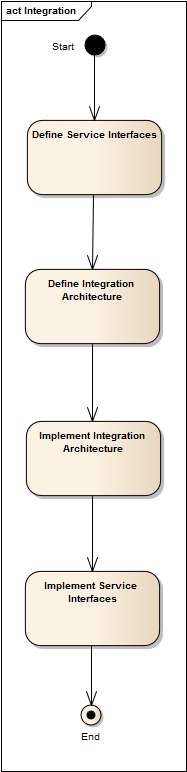
\includegraphics[width=0.3\textwidth]{ch6_activity_integration} 
	\caption{\ac{UML} Activity Diagram: Implement Integration} 
	\label{fig:ch6_activiy_integration} 
\end{figure}

\subsection{Implement Aggregation}
This process is concerned with the implementation of the message aggregation, as shown in the \ac{UML} activity diagram in Figure \ref{fig:ch6_activiy_aggregation}.

\begin{figure}[htpb] \centering 
	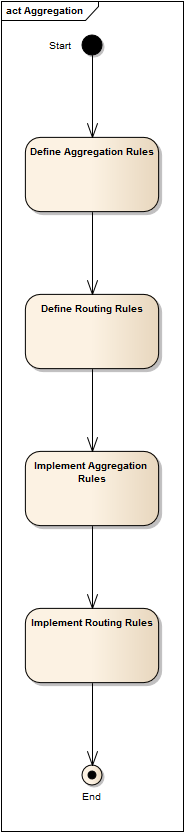
\includegraphics[width=0.3\textwidth]{ch6_activity_aggregation} 
	\caption{\ac{UML} Activity Diagram: Implement Aggregation} 
	\label{fig:ch6_activiy_aggregation} 
\end{figure}

\subsection{Implement Feedback-Control}

This process contains tasks that are concerned with the design, implementation and tuning of the feedback-control loop, as shown in Figure \ref{fig:ch6_tasks_feedback_control}.

\begin{figure}[htpb] \centering 
	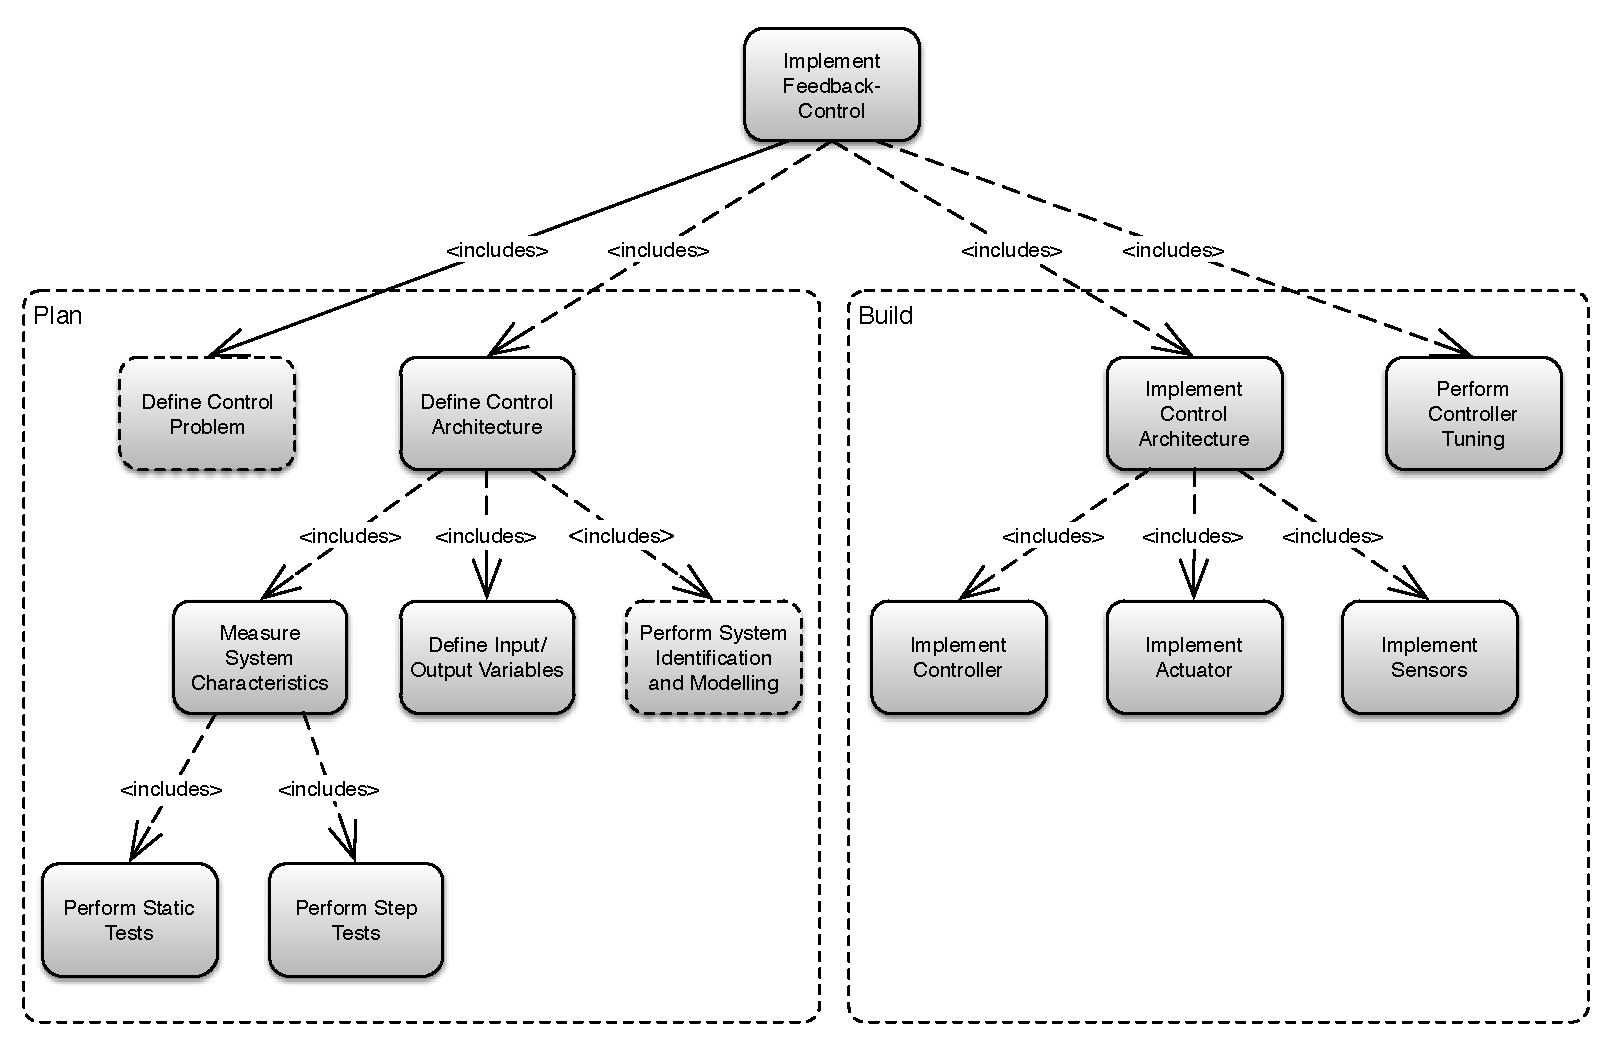
\includegraphics[width=\textwidth]{ch6_tasks_feedback_control} 
	\caption{Tasks for implementing the feedback-control loop} 
	\label{fig:ch6_tasks_feedback_control} 
\end{figure}

There are two options for implementing the feedback-control loop:
\begin{itemize}
	\item Using a system model for performing the controller tuning, as shown in the \ac{UML} activity diagram in Figure \ref{fig:ch6_activiy_feedback_control_model}.
	\item Without using a model, the control architecture needs to be implemented prior to the controller tuning, as shown in the \ac{UML} diagram in Figure \ref{fig:ch6_activiy_feedback_control}.
\end{itemize}

\begin{figure}[htpb] \centering 
	\subfloat[Using a model]{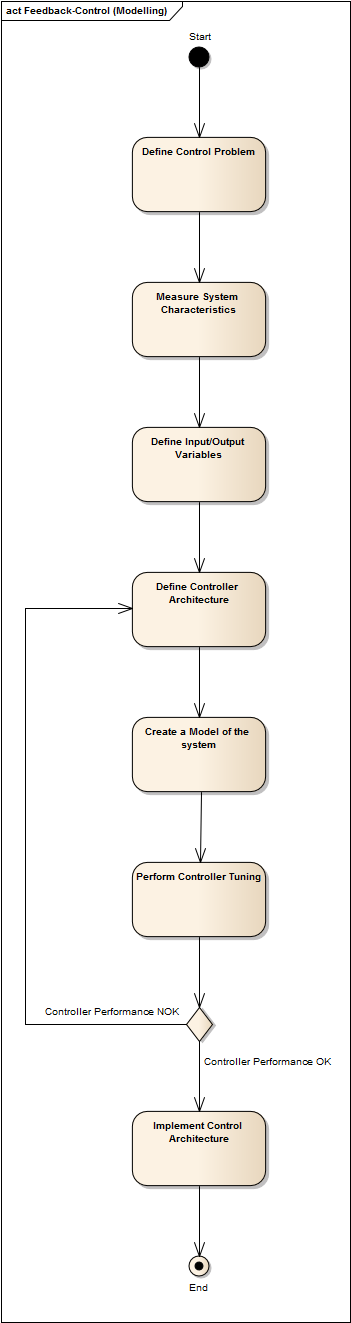
\includegraphics[width=0.3\textwidth]{ch6_activity_feedback_control_modelling}\label{fig:ch6_activiy_feedback_control_model}}\qquad
	\subfloat[Without a model]{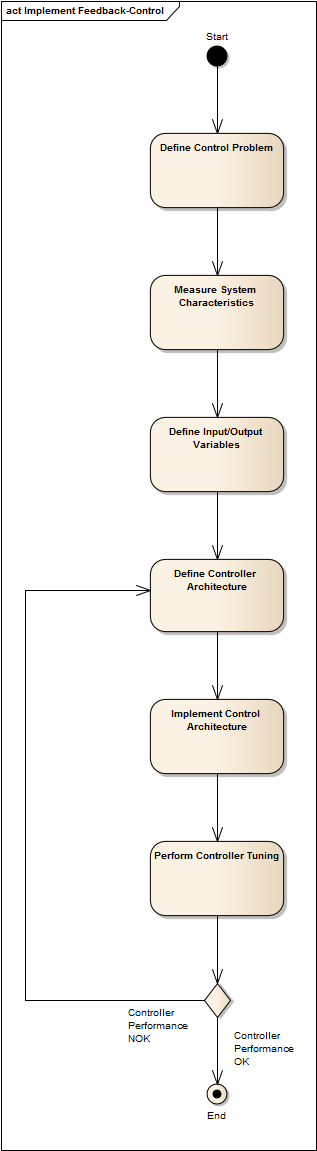
\includegraphics[width=0.3\textwidth]{ch6_activity_feedback_control}\label{fig:ch6_activiy_feedback_control}}
	\caption{\ac{UML} Activity Diagram: Implement Feedback-Control Loop} 
\end{figure}

\section{Artifacts}\label{sec:ch6_artifacts}

An artifact is a result of a task. It is an intermediate result, that is needed for development of the software, but not the software product itself. Additionally, it can also be prerequisite of another task. 

The conceptual framework only describes artifacts that are specific for the implementation of the adaptive middleware as described in Chapter \ref{ch:adaptive_middleware}. Artifacts that are common to every software development process are out of scope.

\begin{figure}[htpb] \centering 
	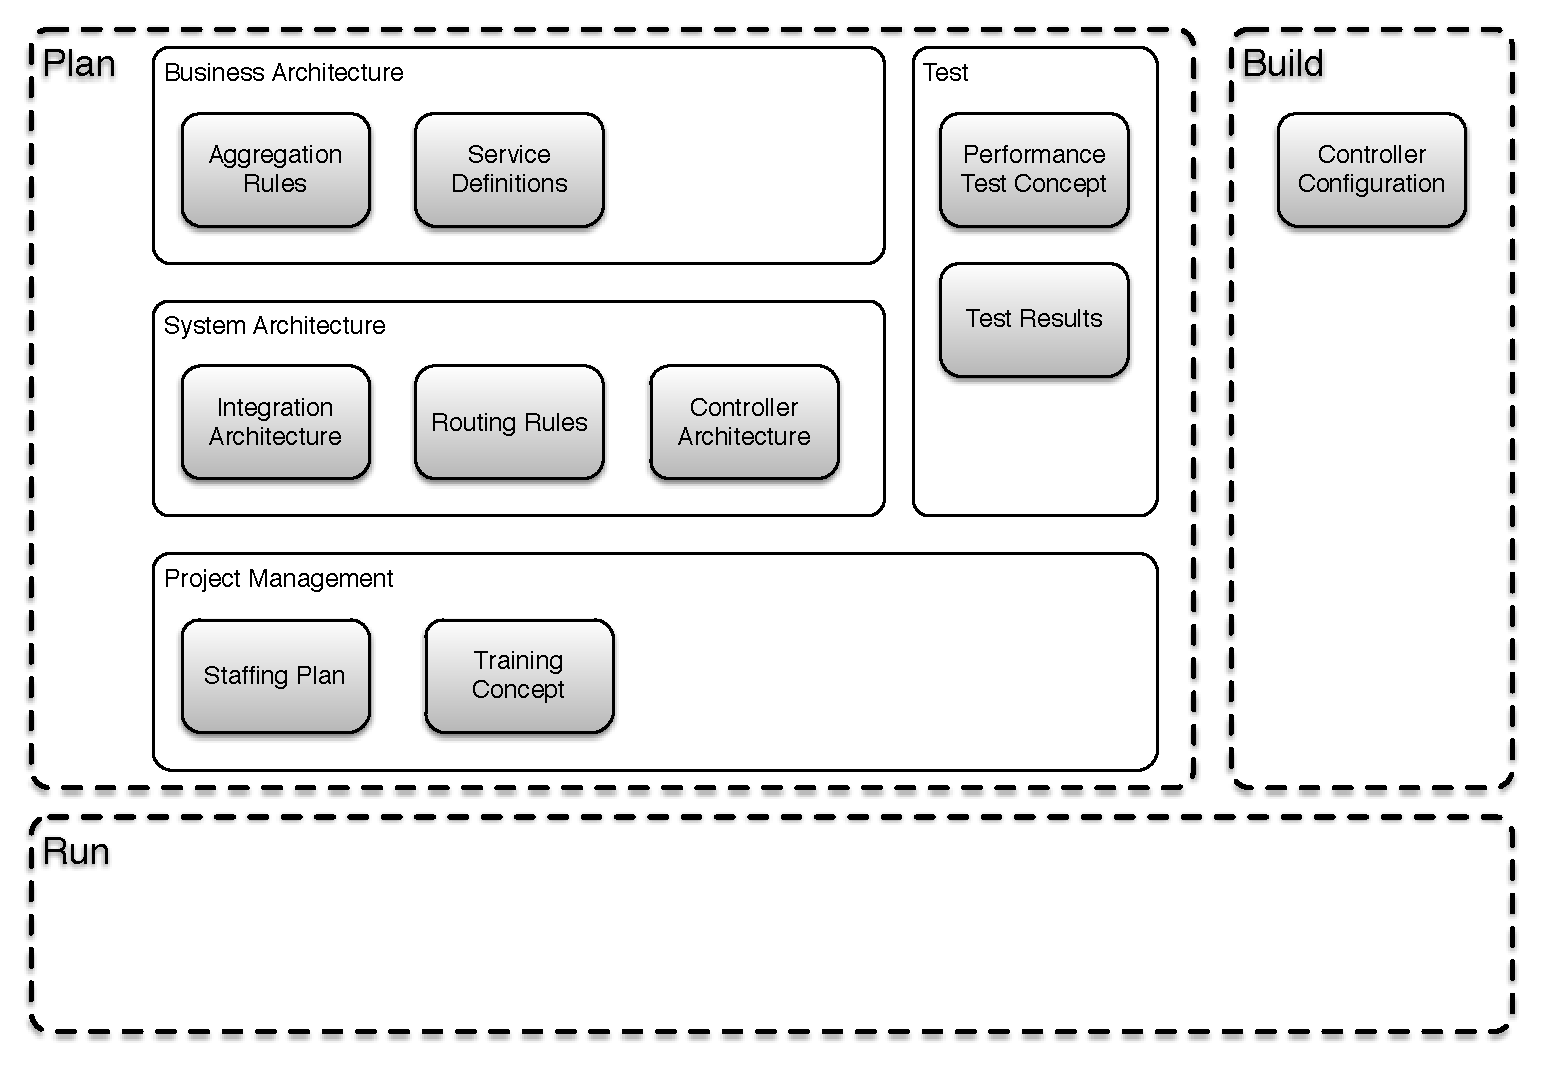
\includegraphics[width=\textwidth]{ch6_artifacts} 
	\caption{Artifacts} 
	\label{fig:ch6_artifacts} 
\end{figure}

The conceptual framework describes the following artifacts:

\begin{itemize}
	\item Performance Requirements
	\item Service Interface Definition
	\item Aggregation Rules
	\item Integration Architecture
	\item Routing Rules
	\item Controller Architecture
	\item System Model
	\item Controller Configuration
	\item Performance Test Concept
	\item Training Concept
	\item Staffing Plan
\end{itemize}

\subsection{Performance Requirements}
\begin{tabularx}{\textwidth}{@{} l X @{}}
	\caption{Performance Requirements} \label{table:ch6_Artifact_Performance_Requirements}\\
	\toprule 
	\bfseries Artifact & Performance Requirements\\
	\midrule 
	\bfseries Description & 
	\begin{itemize}
		\item Defines the structure of input and output data
		\item Does not include informations about the technical format, such as \ac{XML} or \ac{JSON}, and the integration style, such SOAP or \ac{REST}
	\end{itemize}
	\\
	\midrule 
	\bfseries Task & Define Performance Requirements
	\\
	\midrule 
	\bfseries Role & 
	\begin{itemize}
		\item Business Architect
		\item System Architect
	\end{itemize}\\
	\bottomrule 
\end{tabularx}


\subsection{Service Interface Definition}
\begin{tabularx}{\textwidth}{@{} l X @{}}
	\caption{Service Interface Definition} \label{table:ch6_Artifact_Service_Interface_Definition}\\
	\toprule 
	\bfseries Artifact & Service Interface Definition\\
	\midrule 
	\bfseries Description & 
	\begin{itemize}
		\item Defines the structure of input and output data
		\item Does not include informations about the technical format, such as \ac{XML} or \ac{JSON}, and the integration style, such SOAP or \ac{REST}
	\end{itemize}
	\\
	\midrule 
	\bfseries Task & Define Service Interfaces 
	\\
	\midrule 
	\bfseries Role & Business Architect\\
	\bottomrule 
\end{tabularx}

\subsection{Aggregation Rules}

\begin{tabularx}{\textwidth}{@{} l X @{}}
	\caption{Aggregation Rules} \label{table:ch6_Artifact_Aggregation_Rules}\\
	\toprule 
	\bfseries Artifact & Aggregation Rules\\
	\midrule 
	\bfseries Description & Defines how events should be correlated with each other by the Aggregator.\\
	\midrule 
	\bfseries Task & Define Aggregation Rules
		\\
	\midrule 
	\bfseries Role & 
	\begin{itemize}
		\item Business Architect
		\item System Architect
	\end{itemize}
	\\
	\bottomrule 
\end{tabularx}


\subsection{Integration Architecture}

\begin{tabularx}{\textwidth}{@{} l X @{}}
	\caption{Integration Architecture} \label{table:ch6_Artifact_Integration_Architecture}\\
	\toprule 
	\bfseries Artifact & Integration Architecture\\
	\midrule 
	\bfseries Description & Defines the technical integration of the business services, including
	\begin{itemize}
		\item Middleware technology or product
		\item Transports, such as \ac{JMS}, \ac{SOAP} or \ac{FTP}
		\item Technical format of the input and output data, such as \ac{XML} or \ac{JSON}, \ac{CSV} or binary formats.
	\end{itemize}
	\\
	\midrule 
	\bfseries Task & Define Integration Architecture 
		\\
	\midrule 
	\bfseries Role & System Architect\\
	\bottomrule 
\end{tabularx}


\subsection{Routing Rules}

\begin{tabularx}{\textwidth}{@{} l X @{}}
	\caption{Routing Rules} \label{table:ch6_Artifact_Routing_Rules}\\
	\toprule 
	\bfseries Artifact & Routing Rules\\
	\midrule 
	\bfseries Description & Defines which service endpoint should be called by the Router for a given aggregation size.\\
	\midrule 
	\bfseries Task & Define Routing Rules
		\\
	\midrule 
	\bfseries Role & System Architect\\
	\bottomrule 
\end{tabularx}


\subsection{System Model}

\begin{tabularx}{\textwidth}{@{} l X @{}}
	\caption{System Model} \label{table:ch6_Artifact_System_Model}\\
	\toprule 
	\bfseries Artifact & System Model\\
	\midrule 
	\bfseries Description & The system model is used to build a simulation of the system which can be used for implementing the controller.\\
	\midrule 
	\bfseries Task & System Identification / Modelling
	\\
	\midrule 
	\bfseries Role & System Architect\\
	\bottomrule 
\end{tabularx}


\subsection{Controller Configuration}

\begin{tabularx}{\textwidth}{@{} l X @{}}
	\caption{Controller Configuration} \label{table:ch6_Artifact_Controller_Configuration}\\
	\toprule \bfseries Artifact & Controller Configuration\\
	\midrule 
	\bfseries Description & The controller configuration specifies the parameter of the Controller.\\
	\midrule 
	\bfseries Task & Perform Controller Tuning
		\\
	\midrule 
	\bfseries Role & Sofware Engineer\\
	\bottomrule 
\end{tabularx}


\subsection{Training Concept}

\begin{tabularx}{\textwidth}{@{} l X @{}}
	\caption{Training Concept} \label{table:ch6_Artifact_Training_Concept}\\
	\toprule 
	\bfseries Artifact & Training Concept\\
	\midrule 
	\bfseries Description & 
	\begin{itemize}
		\item Defines the audience of the training, for example Operations Engineers, Software Engineers or Test Engineers.
		\item Defines the content of the training, for example basics of control theory, details about the Adaptive Middleware for Bulk Data Processing.
		\item Defines the type of training, such as virtual training, on-site training, face-to-face training. 
		\item Defines a timeplan, learning modules and needed facilities to conduct the training.
	\end{itemize}
	\\
	\midrule 
	\bfseries Task & Define Training Concept
	\\
	\midrule 
	\bfseries Role & 
	\begin{itemize}
		\item Project Manager
		\item System Architect
	\end{itemize}
	\\
	\bottomrule 
\end{tabularx}


\subsection{Staffing Plan}

\begin{tabularx}{\textwidth}{@{} l X @{}}
	\caption{Training Concept} \label{table:ch6_Artifact_Staffing_Plan}\\
	\toprule 
	\bfseries Artifact & Staffing Plan\\
	\midrule 
	\bfseries Description & The staffing plan contains
	\begin{itemize}
		\item The required team members and their utilisation over the project time (staffing curve).
		\item The required roles and their assignment to team members.
		\item A skill matrix that shows the required skills and the knowlegde of each team member.
	\end{itemize}
	\\
	\midrule 
	\bfseries Task & Perform Staffing
	\\
	\midrule 
	\bfseries Role & Project Manager\\
	\bottomrule 
\end{tabularx}


\section{Tools} % (fold)
\label{sec:ch6_tools}

The design and implementation of the adaptive middleware requires the use of some specific tools. Tools are grouped in the following categories:

\begin{itemize}
	\item Tools for system modelling, system identification and simulation
	\item Tool for data visualisation
	\item Tools for data processing
\end{itemize}

\subsection{Tools for System Modelling, System Identification and Simulation}

The implementation of the feedback-controll loop can be aided with special tools for system modelling, system identification or simulation.
Examples of such tools include:

\begin{itemize}
	\item Discrete Event Simulation Frameworks, such as SimPy \citep{simpy}, SystemC \citep{systemc}
	\item MATLAB/Simulink \citep{matlab}
	\item Scilab/Xcos \citep{scilab}
\end{itemize}

\subsection{Tools for Data Visualisation}

In order to gain insights from the performance test  and controller tuning results, the test results should be visualized with a suitable data visualisation tool. Examples of data visualisation tools include:

\begin{itemize}
	\item Microsoft Excel \citep{excel}
	\item MATLAB \citep{matlab}
	\item Gnuplot \citep{gnuplot}
	\item matplotlib \citep{matplotlib}
\end{itemize}

\subsection{Tools for data processing}

For the evaluation of the performance test results, it is often necessary to process log files, which have been generated during the the test runs. For example for the calculation of statistical values. While this can be done with an arbitrary programming language, the following programming or scripting languages are in particular suitable for data processing:

\begin{itemize}
	\item Perl \citep{perl}
	\item Python \citep{python}
\end{itemize}

% section tools (end)

\section{Relationship to Architecture Frameworks and Methodologies} 
\label{sec:ch6_other_frameworks}
% (fold)

The conceptual framework is only concerned with the special aspects of the design, implementation and operation of the adaptive middleware presented in Chapter \ref{ch:adaptive_middleware}. It does not describe a complete software development approach. The conceptual framework therefore needs to be integrated in common software development frameworks or methodologies.

In principle, the conceptual framework can be integrated in any iterative software lifecycle approach, such as the Rational Unified Process, the spiral model \citep{Boehm:1988cd} or agile development frameworks such as Scrum \citep{Schwaber:2013aa}. Linear lifecycle models such as the waterfall model \citep{Royce:1987tl} are not suited because tasks like controller design, controller implementation and controller tuning need to be iterative.

This section describes briefly how the conceptual framework can be used with two common software development methodologies, the \ac{RUP} and Scrum.

\subsection{Rational Unified Process}
The \acf{RUP} is an approach to asssigning activities and responsibilities within a development organization to produce high-quality software that meets the requirements of its users within a predictable schedule and budget \citep{Rational:2001aa}.

\ac{RUP} divides the software lifecycle into cycles, where each cycle is concerned with a new iteration of the software system. A cycle consists of the following phases \citep{Kruchten:1996aa}:

\begin{itemize}
	\item \textbf{Inception}\\
	Establish the business case for the system and define the project scope.
	\item \textbf{Elaboration}\\
	Analyse the the problem domain, establish an architectural foundation and develop the project plan.
	\item \textbf{Construction}\\
	Develop and test the components and application features.
	\item \textbf{Transition}\\
	Transition of the software to its end users.
\end{itemize}

Additionally, \ac{RUP} describes nine core workflows, 6 engineering workflows and 3 supporting workflows:

\begin{itemize}
	\item Engineering workflows
	\begin{itemize}
		\item \textbf{Business modelling workflow}\\
		Documentation of business processes using business use cases.
		\item \textbf{Requirements workflow}\\
		Description of \emph{what} the system should do.
		\item \textbf{Analysis \& Design workflow}\\
		Definition \emph{how} the system  will be realised in the implementation phase.
		\item \textbf{Implementation workflow}\\
		Implementation, unit testing and integration of the system.
		\item \textbf{Test workflow}\\
		Verification that all requirements have been correctly implemented.
		\item \textbf{Deployment workflow}\\
		Production of the product release and delivering the software to its end users.
	\end{itemize}
	\item Supporting workflows
	\begin{itemize}
		\item \textbf{Project Management}\\
		Management of the software development process including its risks.
		\item \textbf{Configuration and Change Management}\\
		Management of the artificats produced by the software development process.
		\item \textbf{Environment}\\
		Provisioning the software development organisation with the software development environment.
	\end{itemize}
\end{itemize}

Figure \ref{fig:ch6_rup} shows the core workflows of the \ac{RUP} and when they are conduction during the different phases.

\begin{figure}[htpb] \centering 
	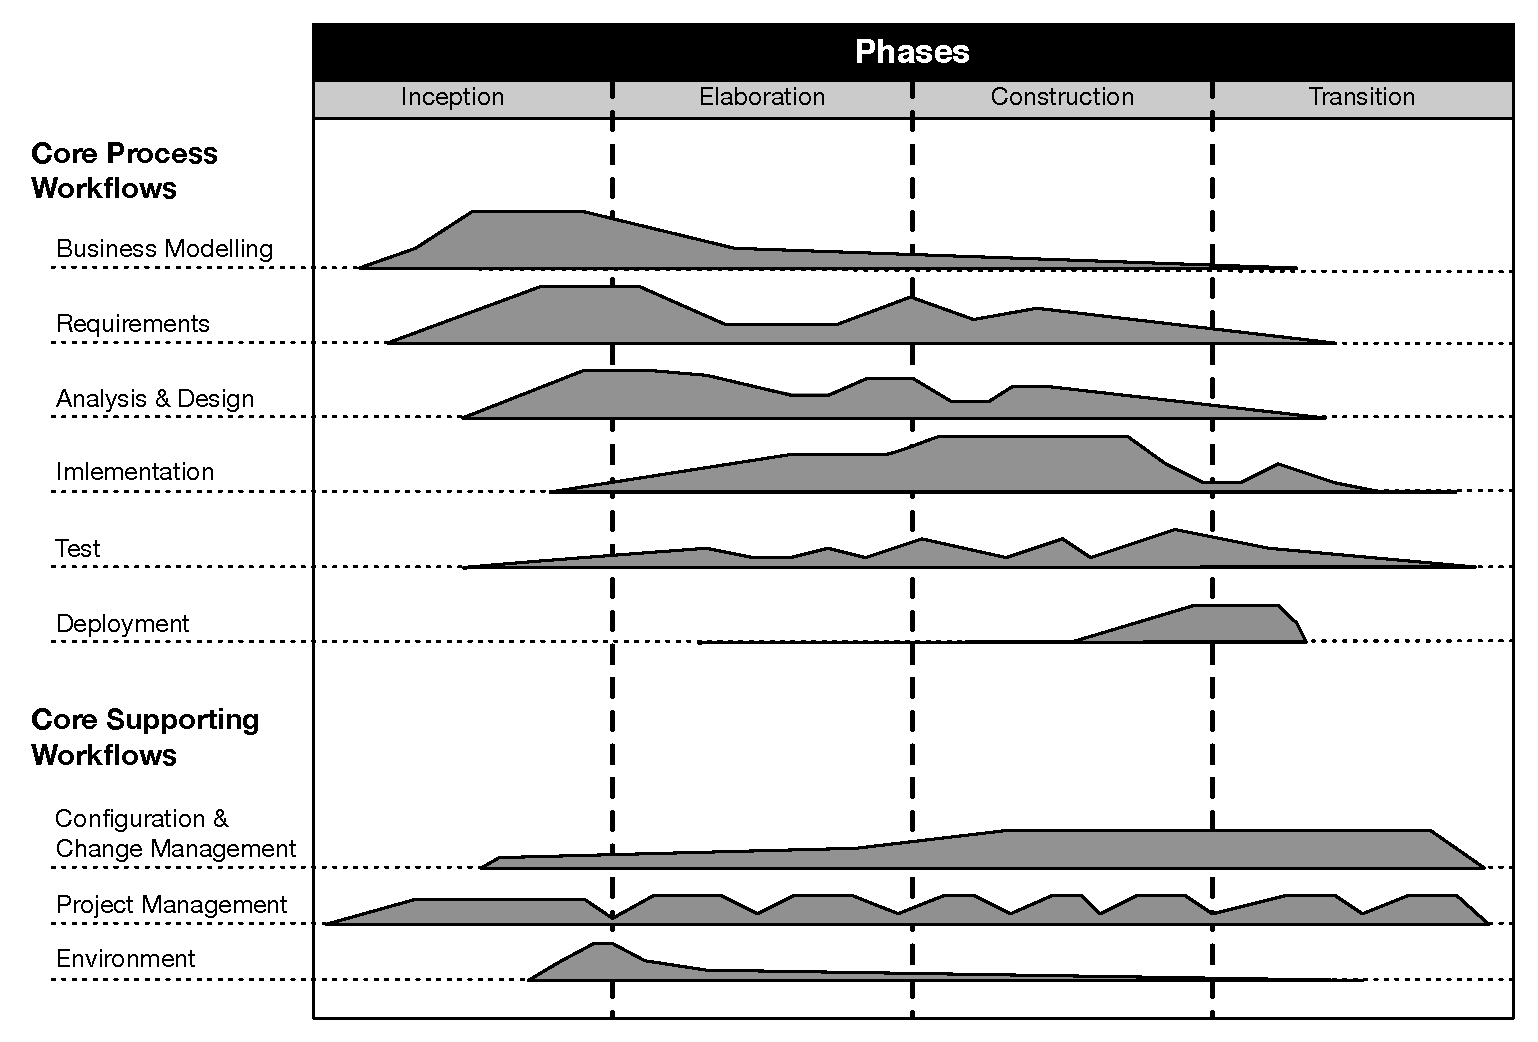
\includegraphics[width=\textwidth]{ch6_rup} 
	\caption{Core process workflows \citep{Kruchten:1996aa}} 
	\label{fig:ch6_rup} 
\end{figure}

The following Table \ref{table:ch6_mapping_rup} shows the assignment of the tasks of the conceptual framework presented in this chapter to the core workflows of the \ac{RUP}.

	\begin{tabularx}{\textwidth}{@{} l X @{}}
		\caption{Mapping of tasks to \acs{RUP} core workflows} \label{table:ch6_mapping_rup}\\
		\toprule
		\bfseries \ac{RUP} core workflow & \bfseries Activity\\
		\midrule
		Business modelling & 
		\begin{itemize}
			\item Define Service Interfaces
			\item Define Aggregation Rules
		\end{itemize}
		\\
		\midrule
		Requirements & 
		\begin{itemize}
			\item Define Performance Requirements
		\end{itemize}
		\\
		\midrule
		Analysis \& Design &
		\begin{itemize}
			\item Define Integration Architeture
			\item Define Routing Rules
			\item Define Controller Architecture
		\end{itemize}
		\\
		\midrule
		Implementation &
		\begin{itemize}
			\item Implement Integration Architecture
			\item Implement Service Interfaces
			\item Implement Aggregation Rules
			\item Implement Routing Rules
			\item Implement Controller
			\item Perform Controller Tuning
		\end{itemize}
		\\
		\midrule
		Test & 
		\begin{itemize}
			\item Define Performance Tests
			\item Evaluate Test Results
			\item Perform Performance Tests
		\end{itemize}
		\\
		\midrule
		Deployment & 
		\begin{itemize}
			\item Setup Monitoring Infrastructure
			\item Setup Test environment
		\end{itemize}
		\\
		\midrule
		Project Management & 
		\begin{itemize}
			\item Perform Staffing
			\item Define Training Concept
		\end{itemize}
		\\
		\midrule
		Environment & 
		\begin{itemize}
			\item Source Project Environments
		\end{itemize}
		\\
		\bottomrule
	\end{tabularx}
	
\subsection{Scrum}
Scrum is a process framework that has been used to manage complex product development \citep{Schwaber:2013aa}. It consists of Scrum Teams and their roles, artifacts, events, and rules. It is an iterative, incremental approach to optimise predictability and control risks by constantely inspecting and adapting the process.

Scrum partitions the development of software products in Sprints, a timeframe of maximum one month during which a usable and potentially releasable software product is created. 

\begin{itemize}
	\item All requirements for the software product are kept in the Product Backlog
	\item The Product Backlog is an ordered list, contains any changes that should be made to the software product
	\item Higher ordered items are more refined than lower items
	\item Evolves during the course of the project, items are added, refined, sorted, estimated
	\item Requirements are sorted according to their business values
	\item Managed by the Product Owner
	\item At the start of each sprint, the Scrum team decides which backlog items should be implemented during this sprint
\end{itemize}

A Backlog item has following properties:
\begin{itemize}
	\item It has a description, order, estimate and value.
	\item It should be possible to be implemented during a single sprint.
	\item Contains all tasks, that are necessary to implement the described feature, such as design, coding, configuration and testing.
	\item Items can be grouped into epics, which represent an important theme of the software product.
\end{itemize}

Table \ref{table:product_backlog} shows an example Backlog containing items for implementing a system based on the adaptive middleware.
Every item contains all the necessary tasks to design, implement and test a feature. For example, the item \emph{REQ-13} contains the tasks define controller architecture, implement control architecture and perform controller tuning.

\begin{landscape}
	\begin{tabularx}{\columnwidth}{@{} l X X X X X @{}}
		\caption{Example Product Backlog} \label{table:product_backlog}\\
		\toprule
		\bfseries ID & \bfseries Priority & \bfseries Description & \bfseries Epic & \bfseries Estimation & \bfseries Status \\
		REQ-5 & 1 & Rating of basic events & Rating Service & 15 & Ready\\
		REQ-6 & 2 & Mediation of basic events & Mediation Service & 10 & Ready\\
		REQ-11 & 3 & Monitoring & Feedback-Control & 10 & Ready\\
		REQ-10 & 4 & Message-Aggregation & Integration Layer & 8 & Ready\\
		REQ-12 & 5 & Message-Routing & Integration Layer & 8 & Ready\\
		REQ-13 & 6 & Basic Controller & Feedback-Control & 10 & Ready\\
		\ldots & \ldots & \ldots & \ldots & \ldots & \ldots\\
		\bottomrule
	\end{tabularx}
\end{landscape}

The Scrum team is self-organised and cross-functional. The team members have all the needed competencies and skill to do their work.
Scrum defines the following roles:
\begin{itemize}
	\item Product Owner
	\begin{itemize}
		\item Responsible for maximising the value of the product and the work of the development team.
	\end{itemize}
	\item Scrum Master
	\begin{itemize}
		\item Ensures that everybody understands the Scrum concepts and that the process is properly enacted.
		\item Coaches the Development team, removes impediments of the Development Team
	\end{itemize}
	\item Development Team
	\begin{itemize}
		\item There are no special roles such as system architect or test engineer.
	\end{itemize}
\end{itemize}

Although Scrum does not define specific roles for the development team, the skills needed for the design and implementation of an enterprise system based on the adapative middleware defined by the conceptual framework need to be considered when staffing the scrum team. 

% section relationship_to_architecture_frameworks_and_methodologies (end)

\section{Related Work}
\label{sec:ch6_related_work}

This section discusses work related to the conceptual framework presented in this chapter. It introduces the terms \emph{Software Process} and \emph{Software Process Modelling} and discusses approaches to model the software process using \ac{UML}.  

\subsection{Software Process}

``The software process is a partially ordered set of activities untertaken to manage, develop and maintain software systems.'' \citep{Acuna:2001aa}

\cite{McChesney:1995aa} describes the software process as ``collection of policies, procedures, and steps undertaken in the transformation of an expressed need for a software product into a software product to meet that need.''.

Another similar definition comes from \cite{Fuggetta:2000ds}. He defines the software process as the ``coherent set of policies, organizational structures, technologies, procedures, and artifacts that are needed to conceive, develop, deploy, and maintain a software product.''

It is necessary to differentiate between the terms software process and software lifecycle. A software lifecycle describes the states through which the software passes from the start of the development until the operation and finally the retirement \citep{Acuna:aa}. 
Examples of software lifecycle models are the waterfall model \citep{Royce:1987tl} oder the spiral model \citep{Boehm:1988cd}.

\subsection{Software Process Modelling}
Software process modelling describes the creation of software development models \citep{Acuna:2001aa}. \cite{Feiler:1993aa} describes the software process model as ``an abstract representation  of a process architecture, process design or process definition, where each of these describe, at various levels of detail, an organization of process elements of either a completed, current or proposed software process.''

Process models are described using \acp{PML}. A \ac{PML} is defined in terms of a notation, a syntax and semantics, often suitable for computational processing \citep{Bendraou:2005dv}.

\cite{Fuggetta:2000ds} describes different purposes of process models:
\begin{itemize}
	\item Process understanding
	\item Process design
	\item Training and education
	\item Process simulation  optimization
	\item Process support
\end{itemize}

Typical elements of \acp{PML} are (see for example \cite{Benali:1992gq}, \cite{Acuna:2001aa}, \cite{Fuggetta:2000ds} and \cite{Curtis:1992kf}):
\begin{itemize}
	\item Agent or Actor
	\item Role
	\item Activity
	\item Artefact or Product
	\item Tools 
\end{itemize}

Process models typically answer the following questions \citep{Curtis:1992kf}:
\begin{itemize}
	\item What is going to be done?
	\item Who is going to do it?
	\item When and where will it be done?
	\item How and why will it be done?
	\item Who is dependant on its being done?
\end{itemize}

Additionally, process models commonly use the following perspectives related to these questions:
\begin{itemize}
	\item Functional: what activities are being performed
	\item Behavioral: In which order (when) are activities performed
	\item Organizational: where and by whom is an activity performed
	\item Informational: the entities produced by the process
\end{itemize}

\cite{McChesney:1995aa} provides two main categories of software process models (see also \cite{Acuna:2001aa})
\begin{itemize}
	\item \textbf{Prescriptive}\\
	A prescripte software process model defines the required or recommended means of executing the software development process. It answers the question ``how should the software be developed''.
	\item \textbf{Descriptive}\\
	A descriptive software process model describes an existing process model. It answers the question ``how has the software been developed''.
\end{itemize}

Examples of software process models include the IEEE and ISO standards IEEE 1974-1991, ISO/IEC 12207 and the \acf{RUP}.

\subsection{Software Process Modelling using \ac{UML}}
\ac{UML} is commonly used for modelling software processes. 

\ac{UML4SPM} is an \ac{UML}-based metamodel for software process modelling \citep{Bendraou:2005dv,Bendraou:2006aa}. It takes advantages of the expressiveness of \ac{UML} 2.0 by extending a subset of its elements suitable for process modelling. \ac{UML4SPM} contains two packages. The process structure package, which contains the set of primary process elements and the foundation package, which contains the subset of \ac{UML} 2.0 concepts extended by this process elements to provide concepts and mechanisms for the coordination and execution of activities.

\ac{SPEM} 2.0 is a metamodel for modeling software development processes and a conceptual framework, which provides concepts for for modeling, documenting, presenting, managing, interchanging, and enacting development methods and processes \citep{Group:2008aa}. It provides a clear separation between method content, for example deliverables and key roles, and workflows supporting different software lifecycle models. The \ac{SPEM} 2.0 metamodel consists of seven main metamodel packages, with each package extending the package it depends on:
\begin{itemize}
	\item \textbf{Core}\\
	Contains common classes and abstractions as the base for classes in all other packages.
	\item \textbf{Process Structure}\\
	Defines the base for all process models.
	\item \textbf{Process Behaviour}\\
	Extends the concepts of the process structure package with behavioural models.
	\item \textbf{Managed Content}\\
	Contains concepts for managing the textual content of natural language documentation.
	\item \textbf{Method Content}\\
	Provides concepts to build up development knowledge base independent of any specific processes and development projects.
	\item \textbf{Process With Methods}\\
	Defines structures for integrating processes defined with concepts of process structure package with instances of concepts of the method content package.
	\item \textbf{Method Plugin}\\
	Contains concepts for designing and managing maintainable, large scale, reusable, and configurable libraries or repositories of method content and processes.
\end{itemize}

Both approaches, \ac{UML4SPM} and \ac{SPEM} 2.0 extend the \ac{UML} 2.0 notation with additional elements, which does not allow the usage of standard \ac{UML} tools.

\cite{Dietrich:2013aa} use \ac{UML} 2.0 for modelling software processes at Siemens AG. According to the authors, the usage of standard UML 2.0 notation, which is supported by standard modelling tools, increases readability of processes for software developers since UML is also used for modelling the software itself.
They describe four distinct process views: 
\begin{itemize}
	\item Process-oriented view
	\item Activity-oriented view
	\item Product-oriented view
	\item Role-oriented view
\end{itemize}

The following UML diagram types are used by their approach: 
\begin{itemize}
	\item Activity diagrams (process-oriented view)
	\item Class diagrams (activity-oriented view, product-oriented view, role-oriented view)
	\item Use-case diagrams (activity-oriented view, product-oriented view, role-oriented view)
\end{itemize} 

The conceptual framework for feedback-controlled systems for bulk data processing presented in this chapter is based on the properties of the described approaches in this section for modelling the software development process. It uses standard \ac{UML} use-case and activity diagrams for describing tasks and processes for the following reasons:
\begin{itemize}
	\item \textbf{Understandability}\\
	Using standard \ac{UML} 2.0 notation elements and diagrams facilitate the understanding of the conceptual framework since they are commonly used by software engineers for the design of the software system itself. 
	\item \ac{Tool support}\\
	Standard \ac{UML} 2.0 notation elements and diagrams are supported by a wide range of modelling tools.
\end{itemize}

Standard metamodels for software process modelling such as \ac{SPEM} 2.0 have not been used because they seemed to heavyweight for this purpose.

\section{Summary}
\label{sec:ch6_summary}
In this chapter a conceptual framework has been presented to guide the design, implementation and operation of an enterprise system that implements the adaptive middleware for bulk data processing as described in the previous Chapter \ref{ch:adaptive_middleware}.

The conceptual consists of the entities phases, roles, tasks, artifacts and tools. It describes:
\begin{itemize}
	\item The needed roles and their skills for the design, implementation and operation.
	\item The necessary tasks and their relationships for the design, implementation and operation.
	\item The artifacts that are created and required by the different tasks.
	\item The tools that are needed to process the different tasks.
	\item The processes that describe the order of tasks to implement a certain feature of the software system.
\end{itemize}



It should be noted that software processes are not fixed during their lifetime, they need to be continuously improved. \citep{Fuggetta:2000ds}
The conceptual model can therefore be tailored to specific projects requirements, it does not have to be followed strictly.
